\documentclass[11pt]{article}
% Shared preamble for the research-note series.
% Create note-specific content in the per-note directory; keep common macros here.
\usepackage[margin=1in]{geometry}
\usepackage[T1]{fontenc}
\usepackage[utf8]{inputenc}
\usepackage{amsmath,amssymb}
\usepackage{booktabs,longtable,array}
\usepackage{graphicx}
\usepackage{float}
\usepackage{enumitem}
\usepackage{xcolor}
\usepackage{hyperref}
\usepackage{caption}
\usepackage{titlesec}
\hypersetup{colorlinks=true, linkcolor=blue!60!black, urlcolor=blue!60!black, citecolor=blue!60!black}
\setlist[itemize]{leftmargin=1.25em, itemsep=0.2em, topsep=0.3em}
\setlist[enumerate]{leftmargin=1.4em, itemsep=0.2em, topsep=0.3em}
\setlength{\parindent}{0pt}
\setlength{\parskip}{0.6em}
\newcommand{\statusbox}[2]{%
  \noindent\fcolorbox{black}{gray!10}{%
    \parbox{\dimexpr\linewidth-2\fboxsep-2\fboxrule\relax}{%
      \textbf{Status:} #1\\#2
    }%
  }
}

% Shared notation helpers for the research-note series.
\newcommand{\Jlin}{J}
\newcommand{\Jphys}{J_{\mathrm{phys}}}
\newcommand{\Jsurf}{J_{\mathrm{surf}}}
\newcommand{\JdB}{J_{\mathrm{dB}}}
\newcommand{\phiopt}{\phi_{\mathrm{opt}}}
\newcommand{\sigmathreedb}{\sigma_{3\mathrm{dB}}}
\newcommand{\Nt}{N_t}
\newcommand{\Nphi}{N_{\phi}}
\newcommand{\Lfiber}{L}
\newcommand{\Pcont}{P}
\newcommand{\band}{\mathcal{B}_{\mathrm{Raman}}}
\newcommand{\todoitem}[1]{\textcolor{red!70!black}{\textbf{TODO:} #1}}


\usepackage{tabularx}
\usepackage{placeins}

\title{Long-Fiber Single-Mode Raman Suppression}
\author{Fiber Raman Suppression Project}
\date{Evidence snapshot: 2026-04-28}

\begin{document}
\maketitle

\begin{abstract}
This note summarizes the single-mode long-fiber Raman-suppression lane. The
main result is that the project can run checkpointed 100--200 m SMF-style
optimizations and produce image-backed suppression near \(-55\,\mathrm{dB}\)
from almost unshaped Raman transfer. The important caveat is that these are
completed long-fiber milestones, not converged global optima. The current
value of the lane is practical and scientific: it shows how short-fiber phase
structure can seed much longer propagation, how the grid/checkpoint workflow
must change, and where the remaining convergence and lab-readiness gaps are.
\end{abstract}

\section*{Claim Status}
\statusbox{completed milestone with convergence caveats}{The 100 m and 200 m
single-mode result artifacts have complete standard images and strong scalar
suppression. They should be presented as supported exploratory long-fiber
simulation results, not as final optimized lab waveforms.}

\section{Question and Thesis}

The short-fiber baseline asks whether input spectral phase can suppress Raman
transfer over a few meters. The long-fiber question is harder:
\[
    \text{Can the same phase-only control idea still work over }100\text{--}200\,\mathrm{m}?
\]

The answer is yes, with caveats. The result is not a clean theorem that one
phase profile works for every long fiber. It is a computational finding:
with explicit long-fiber grids, warm starts, checkpointed L-BFGS, and standard
image inspection, the project can reach deep Raman suppression in 100--200 m
single-mode simulations.

\begin{figure}[H]
\centering
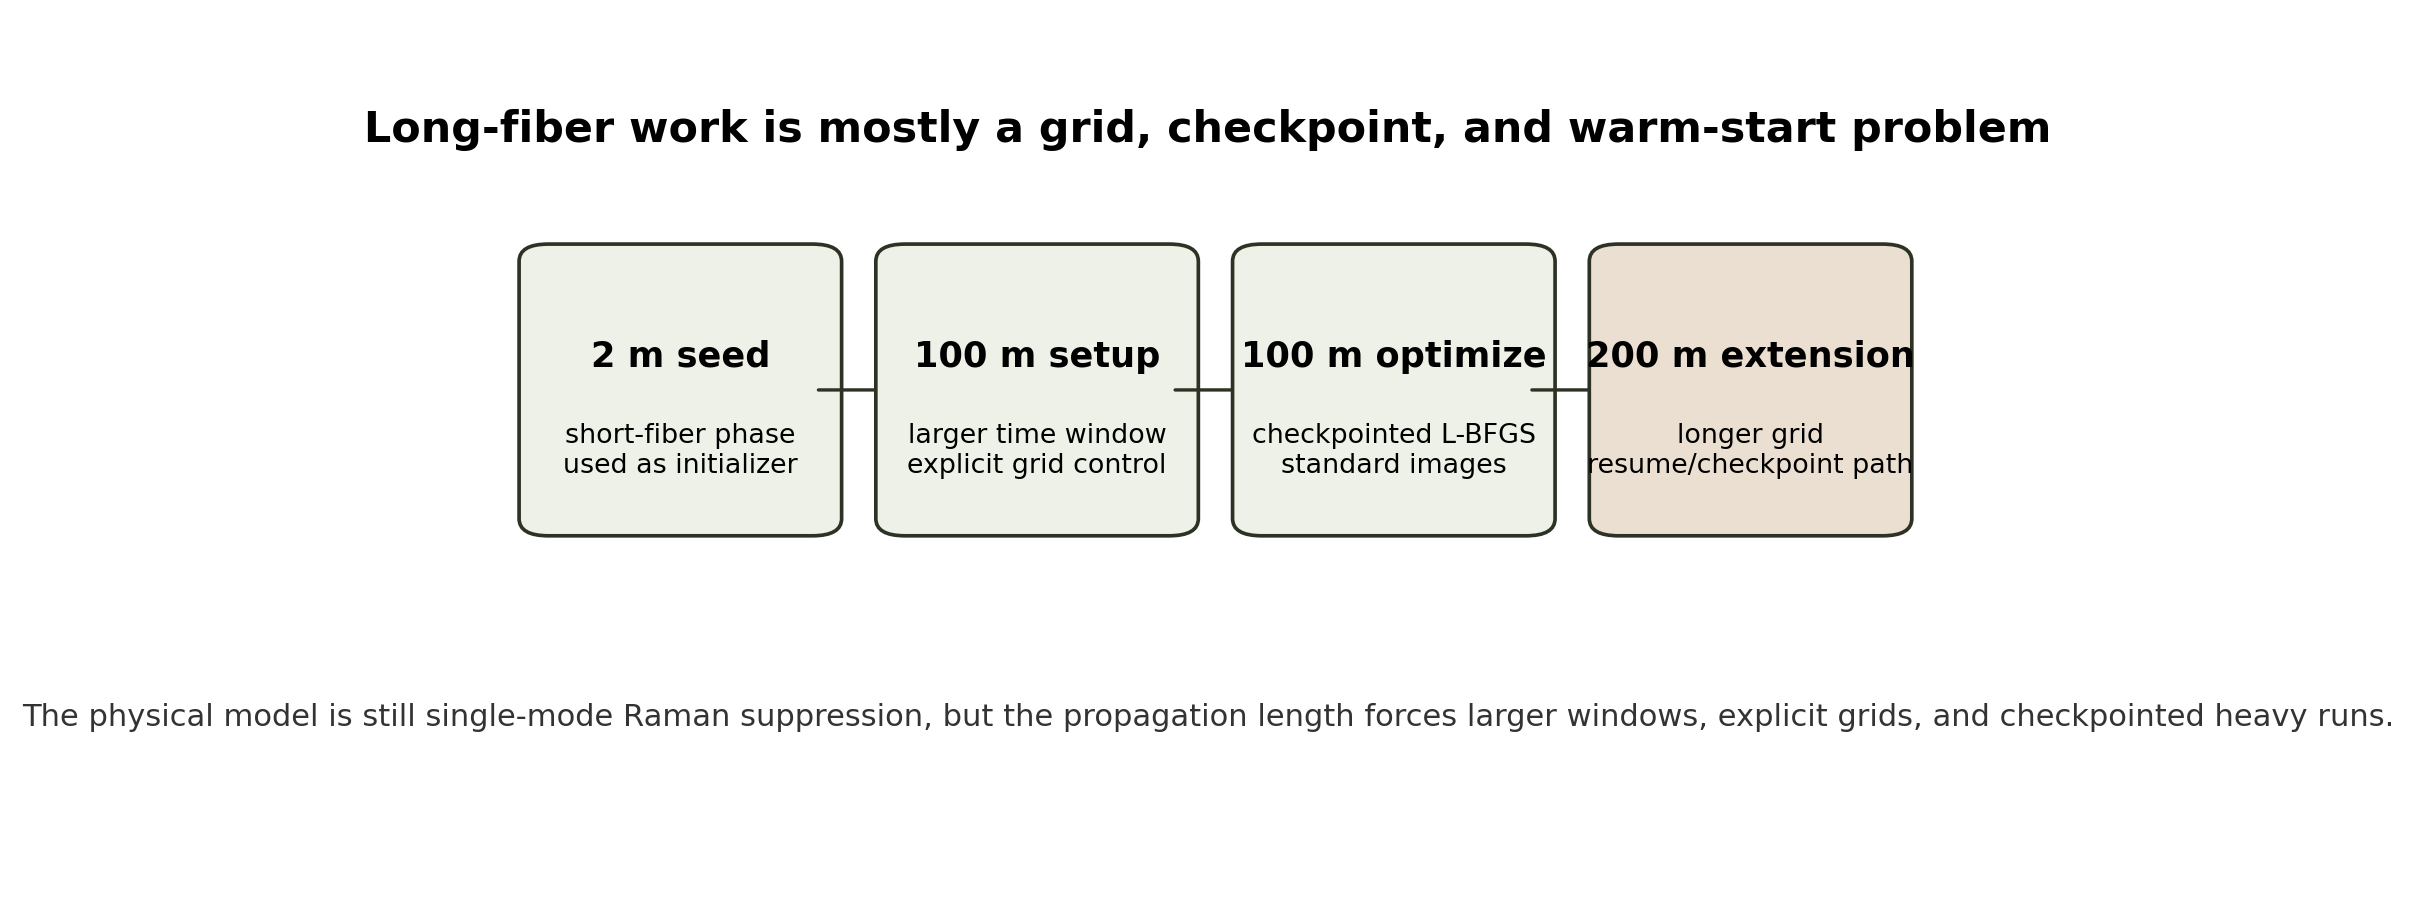
\includegraphics[width=0.95\linewidth]{figures/longfiber_workflow.png}
\caption{Long-fiber optimization changes the compute and validation workflow
more than the physics objective. The solver still optimizes input spectral
phase, but the run needs larger windows, explicit grids, warm starts, and
checkpoint/restart support.}
\end{figure}

\section{Cost Function and Model}

The physical objective is the same Raman-band fraction used in the baseline
note:
\[
    J_{\mathrm{R}}(\phi)=
    \frac{\sum_{\omega_k\in\band}|\hat u_k(L;\phi)|^2}
         {\sum_k |\hat u_k(L;\phi)|^2}.
\]
The input is phase-only:
\[
    \hat u_k(0;\phi)=\hat u_{0,k}e^{i\phi_k}.
\]
The reported scalar is
\[
    J_{\mathrm{dB}}=10\log_{10} J_{\mathrm{R}}.
\]
More negative is better.

The propagation model is the single-mode nonlinear fiber model used elsewhere
in the project: dispersion, Kerr nonlinearity, and Raman response in the
generalized nonlinear Schr\"odinger-equation family. This is standard nonlinear
fiber-optics modeling territory \cite{agrawal2019,dudley2006}. The numerical
approach follows interaction-picture fiber propagation practice
\cite{hult2007}.

\subsection*{TL;DR for the Math}

Nothing magical happens to the objective when the fiber becomes long. The same
fraction is being minimized. What changes is that the pulse has much more
distance to disperse, Raman shift, and develop numerical boundary risk. So the
main mathematical danger is not redefining the cost; it is using a grid too
small to represent the long propagation honestly.

\section{Long-Fiber Grid and Checkpoint Strategy}

Short-fiber runs can often use compact grids. Long-fiber runs cannot blindly
reuse those settings because dispersion walk-off and nonlinear reshaping spread
the pulse over a wider temporal interval. The long-fiber setup therefore
honors the requested \((N_t,\mathrm{time\ window})\) pair instead of letting the
short-fiber setup silently resize it.

\begin{figure}[H]
\centering
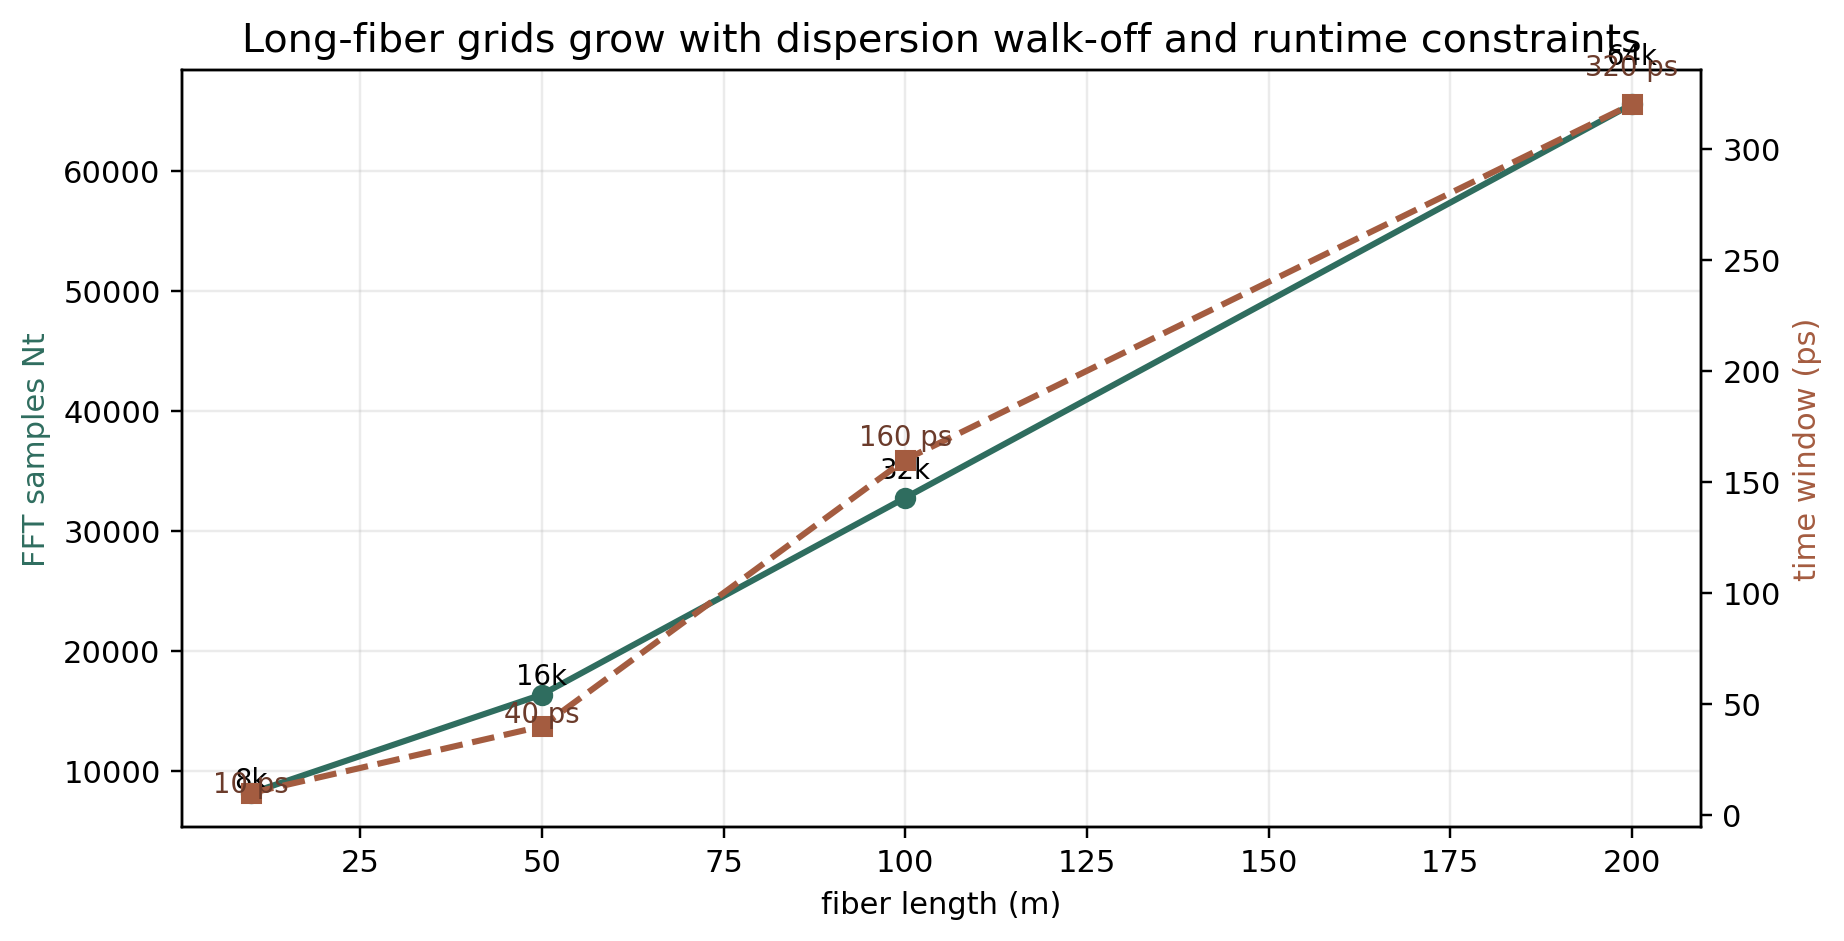
\includegraphics[width=0.82\linewidth]{figures/longfiber_grid_ladder.png}
\caption{Recommended long-fiber grid ladder used by the research scripts. The
200 m run used \(N_t=65536\) and a \(320\,\mathrm{ps}\) time window.}
\end{figure}

The long-fiber optimizer also writes checkpoints. This matters because a 100 m
or 200 m solve is expensive enough that losing the process should not lose the
research state. The key operational pattern is:
\[
    \text{warm start} \rightarrow \text{checkpointed L-BFGS}
    \rightarrow \text{resume if needed} \rightarrow \text{standard images}.
\]

\subsection*{Implementation Surface}
\begin{tabularx}{\linewidth}{@{}p{0.34\linewidth}X@{}}
\toprule
\textbf{Component} & \textbf{Role} \\
\midrule
Problem setup & Builds the explicit long-fiber problem and interpolates warm-start phases across grids. \\
Optimization driver & Checkpointed L-BFGS driver used for the 100 m and 200 m single-mode runs. \\
Checkpoint helper & Resume/config-hash guard so long heavy runs can continue safely. \\
Validation helper & Post-run validation and reporting path for accepted long-fiber artifacts. \\
Standard-image helper & Regenerates the phase profile, phase diagnostic, optimized heat map, and unshaped-control heat map from saved results. \\
\bottomrule
\end{tabularx}

\section{Experimental Method}

The long-fiber lane used four checks:
\begin{enumerate}
    \item propagate the flat/no-shaping control;
    \item transfer a strong short-fiber phase profile to the long grid as a warm start;
    \item run checkpointed L-BFGS on the long-fiber objective;
    \item inspect the standard image set: phase profile, phase diagnostic,
    optimized heat map, and unshaped-control heat map.
\end{enumerate}

For the 100 m case, the flat control is about \(-0.20\,\mathrm{dB}\), the
warm-start phase already reaches about \(-51.50\,\mathrm{dB}\), and the long
optimization reaches the \(-55\,\mathrm{dB}\) class. For the 200 m case, the
accepted resumed artifact reaches \(-55.16\,\mathrm{dB}\).

\subsection*{Provenance and Reproducibility Check}

The figures in this note are copied from standard long-fiber image sets: each
accepted result has a phase profile, phase diagnostic, optimized evolution heat
map, and unshaped-control heat map. The numbers should be read together with
the convergence status. A deep final \(\JdB\) value is not enough by itself;
the note also records whether the optimizer converged, what grid was used, and
whether the standard images were visually inspected.

\subsection*{TL;DR}

The evidence is strong enough to present as a long-fiber simulation milestone.
It is not strong enough to call the saved masks globally optimal or lab-ready.
The honest claim is: the workflow scales to 100--200 m, produces deep
image-backed suppression, and exposes the remaining convergence and actuator
readiness gaps.

\begin{figure}[H]
\centering
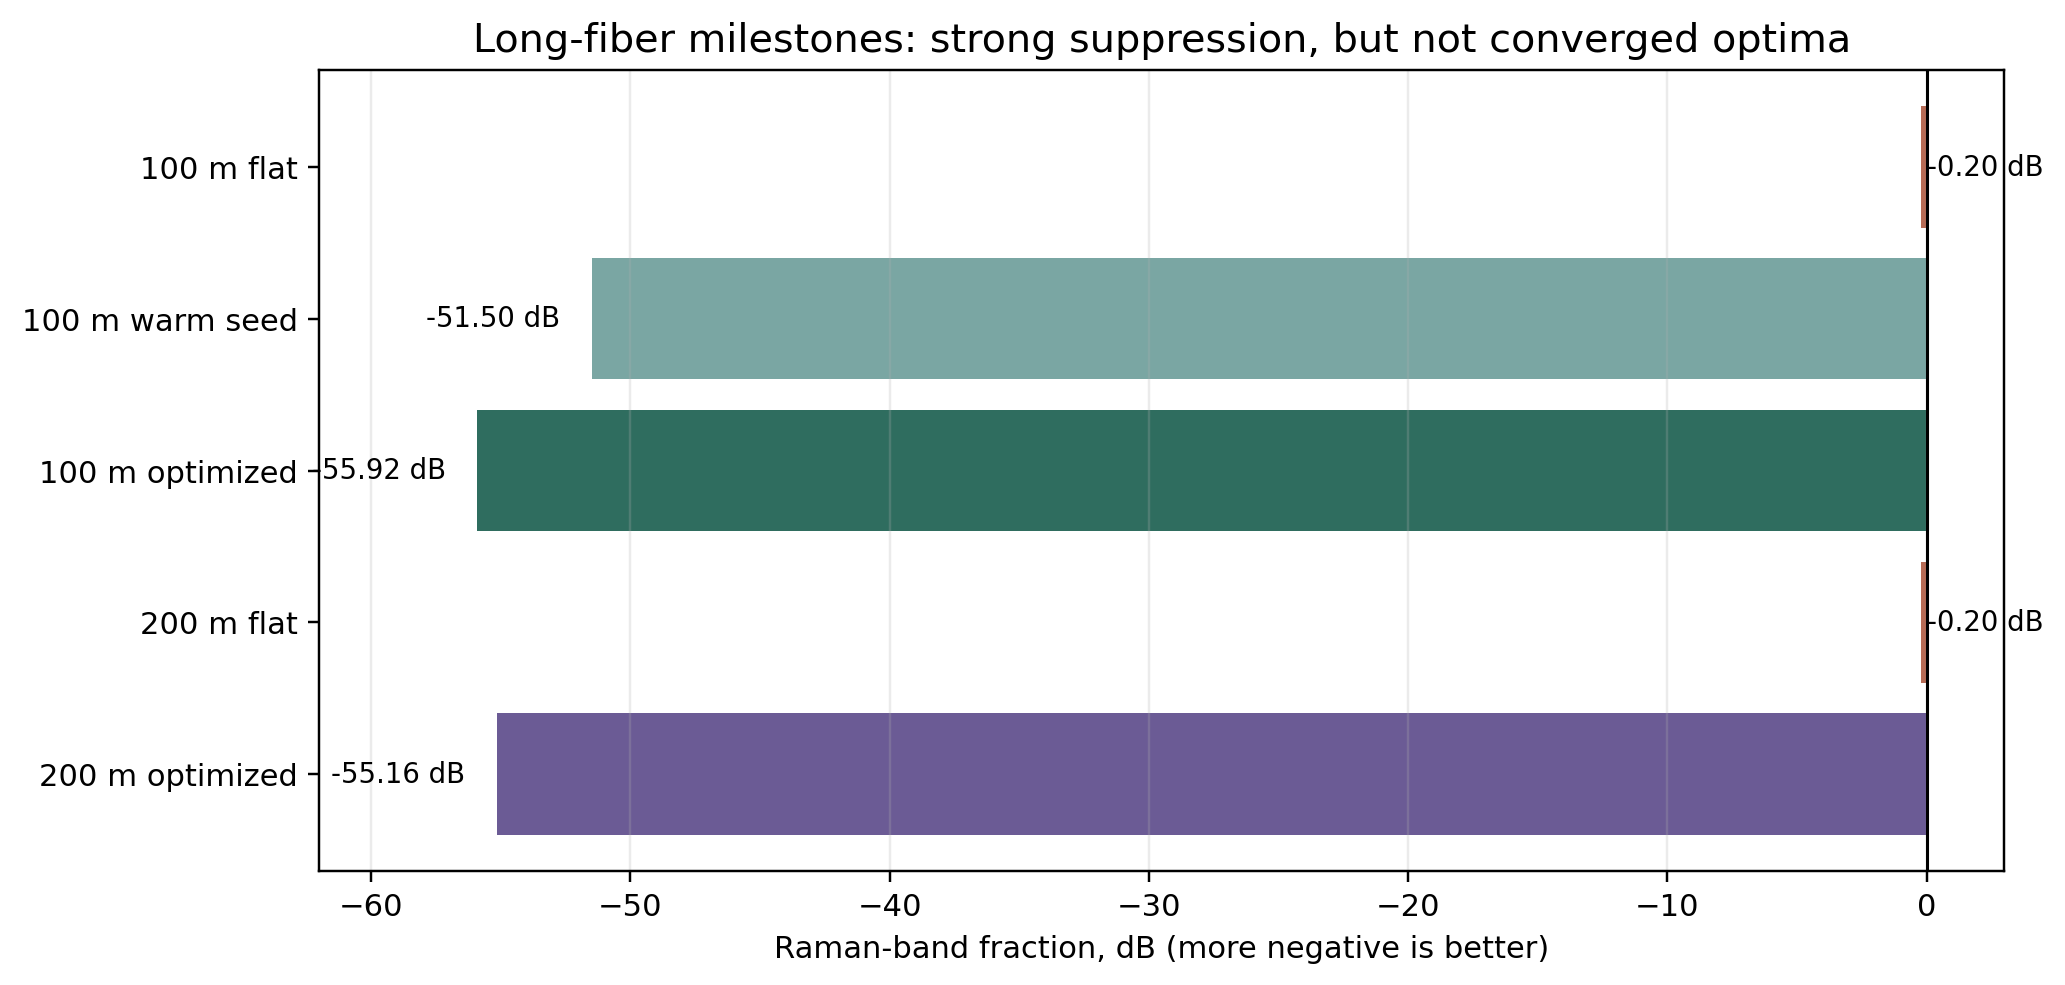
\includegraphics[width=0.88\linewidth]{figures/longfiber_result_summary.png}
\caption{Long-fiber scalar milestones. The 100 m and 200 m optimized results
are deep, image-backed suppression results, but the optimizer convergence flags
remain false.}
\end{figure}

\section{100 m Result}

\begin{figure}[H]
\centering
\begin{minipage}{0.48\linewidth}
\centering
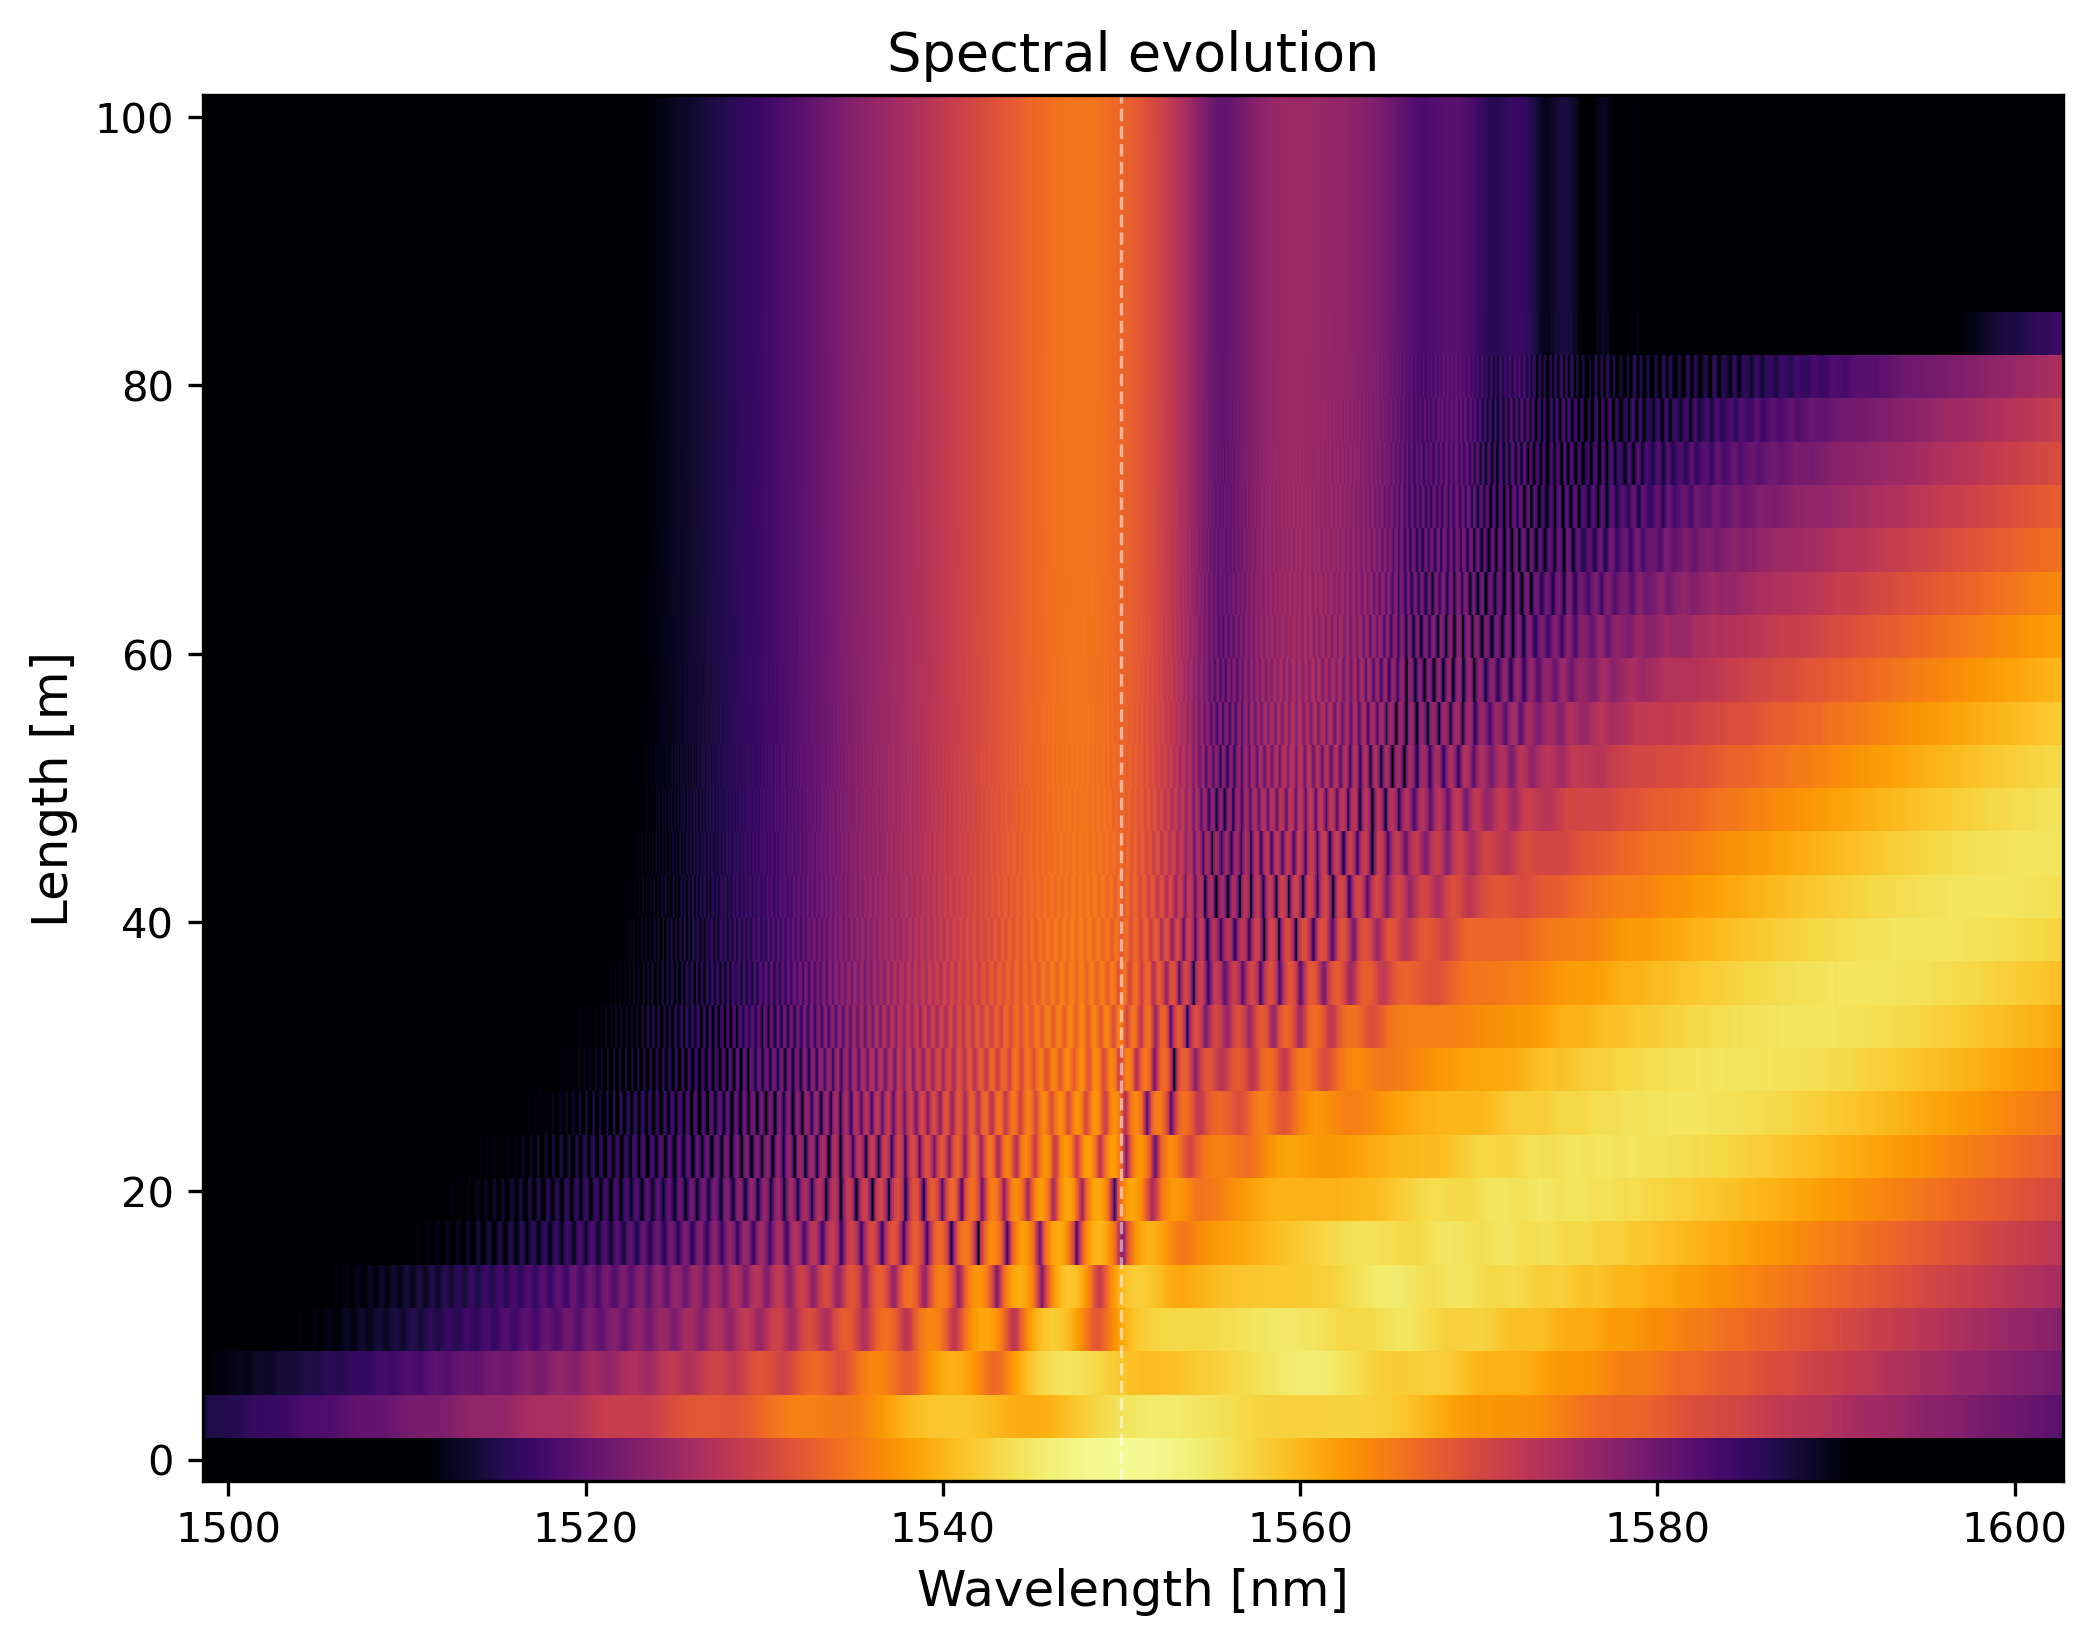
\includegraphics[width=\linewidth]{figures/longfiber_100m_evolution_unshaped.png}
\caption*{100 m no-shaping control.}
\end{minipage}
\hfill
\begin{minipage}{0.48\linewidth}
\centering
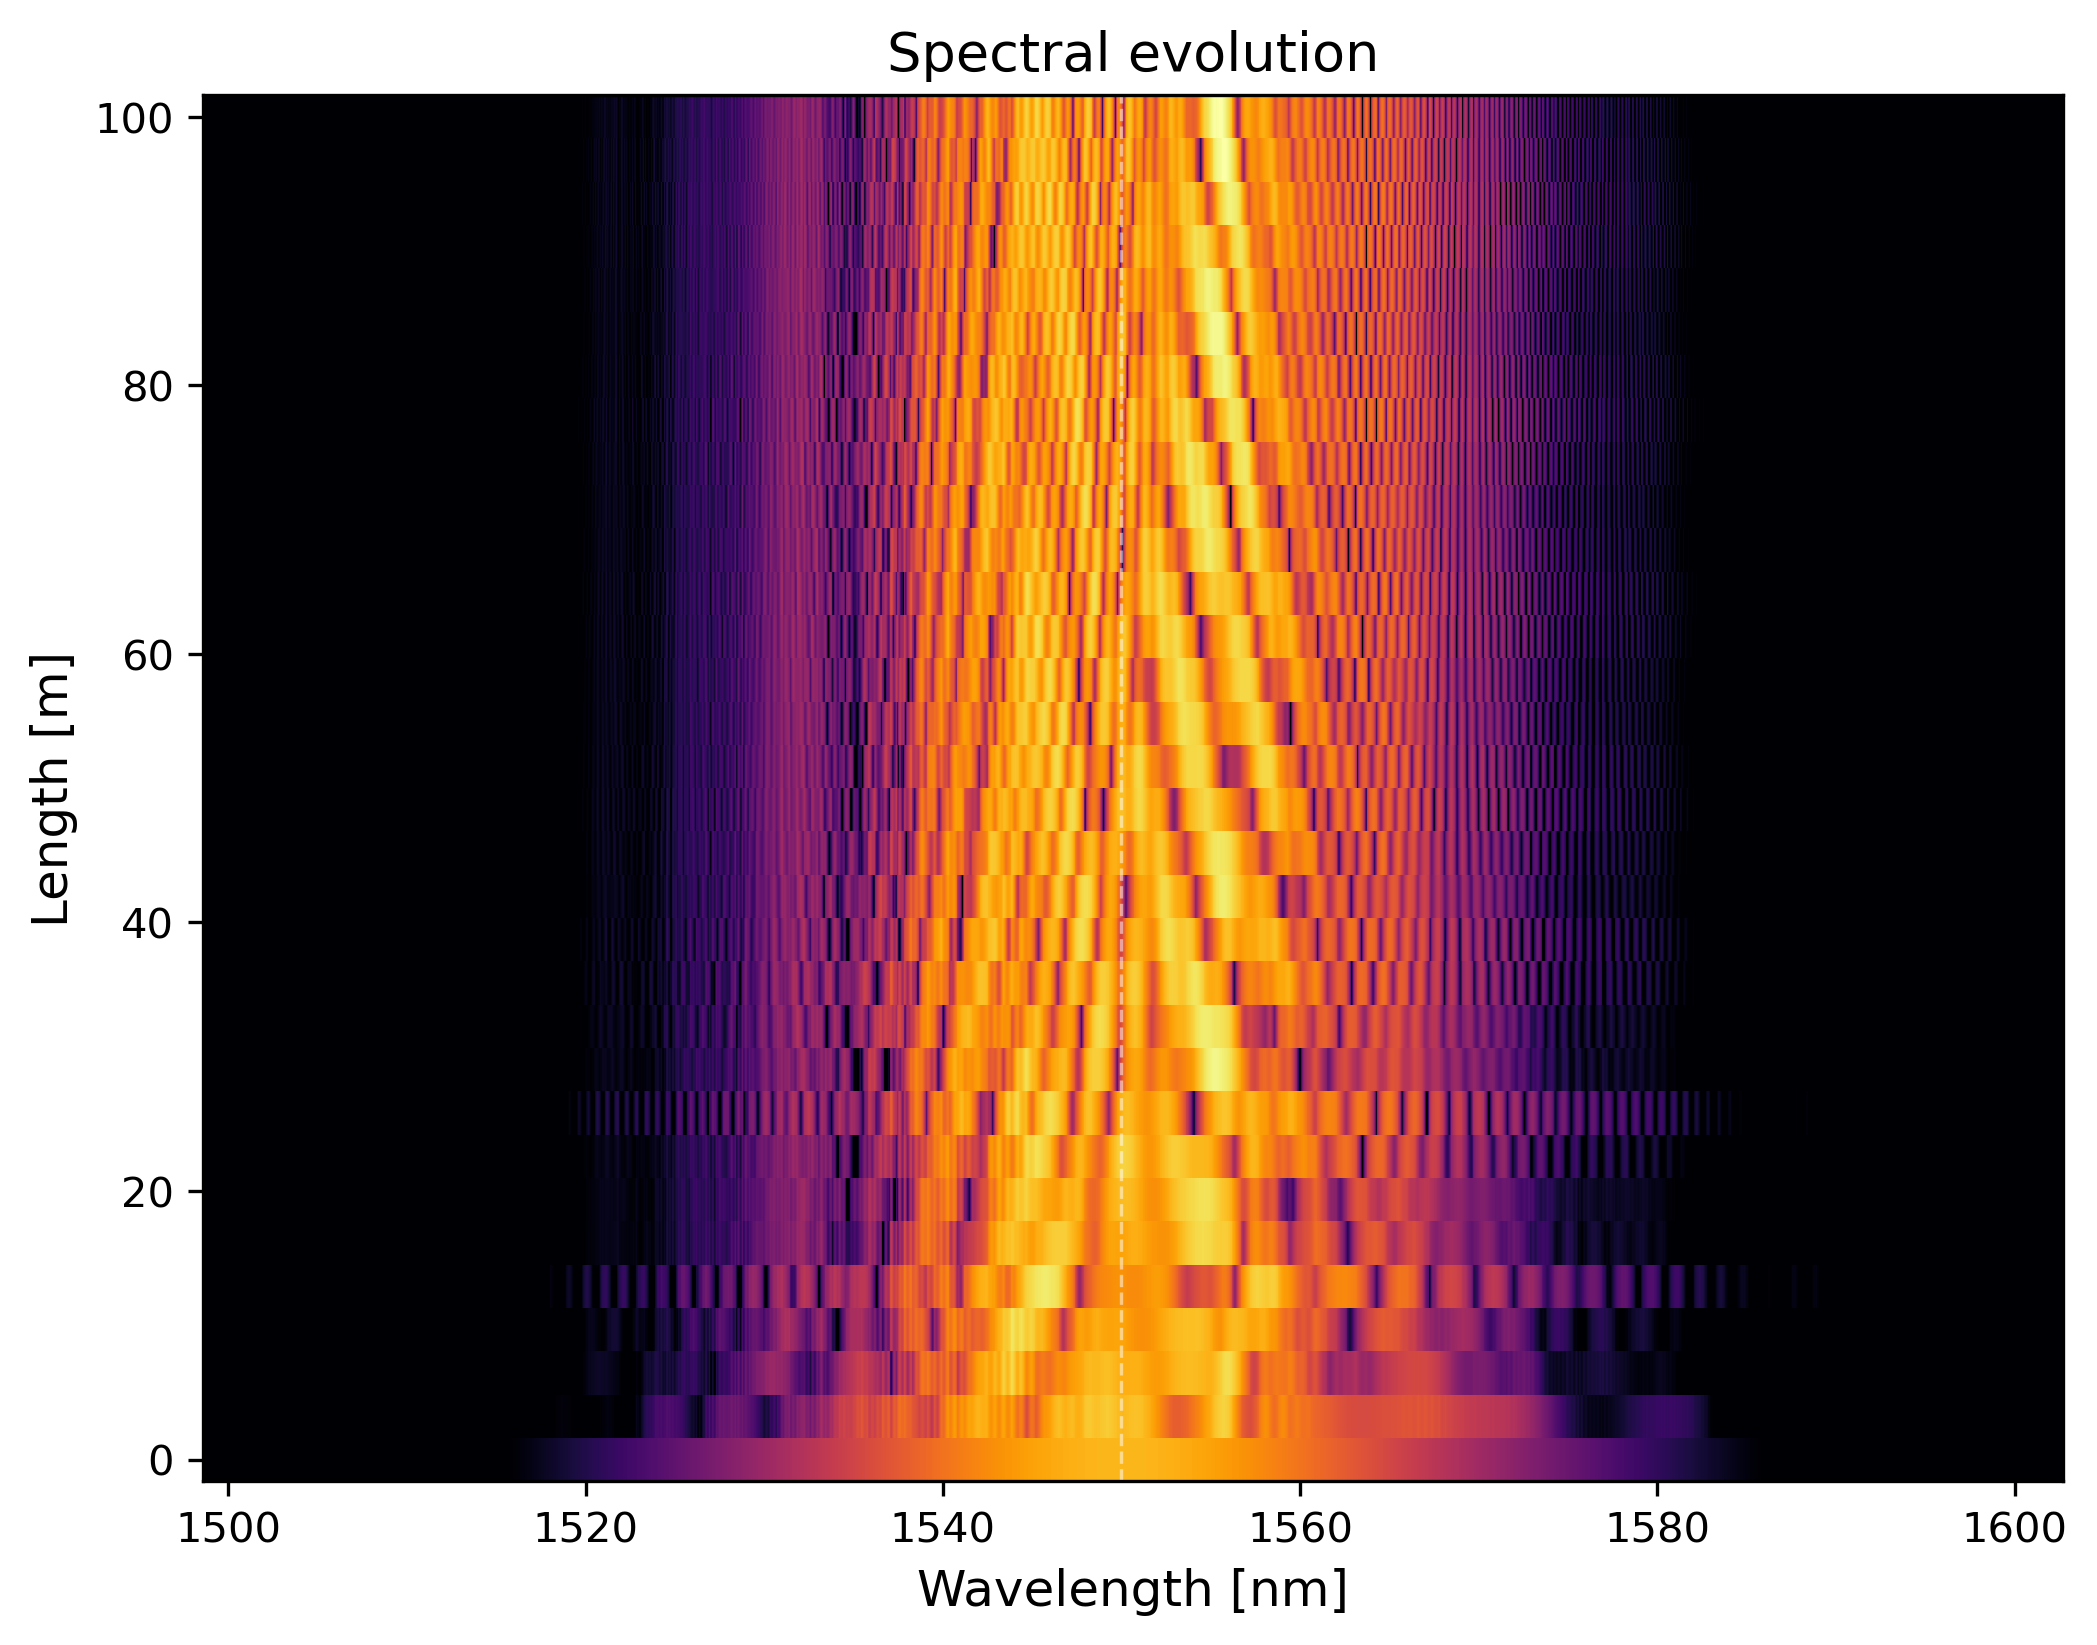
\includegraphics[width=\linewidth]{figures/longfiber_100m_evolution.png}
\caption*{100 m optimized heat map.}
\end{minipage}
\caption{The 100 m comparison is visually strong: the no-shaping control shows
heavy Raman-side growth, while the optimized phase keeps the output mostly near
the input spectral support.}
\end{figure}

\begin{figure}[H]
\centering
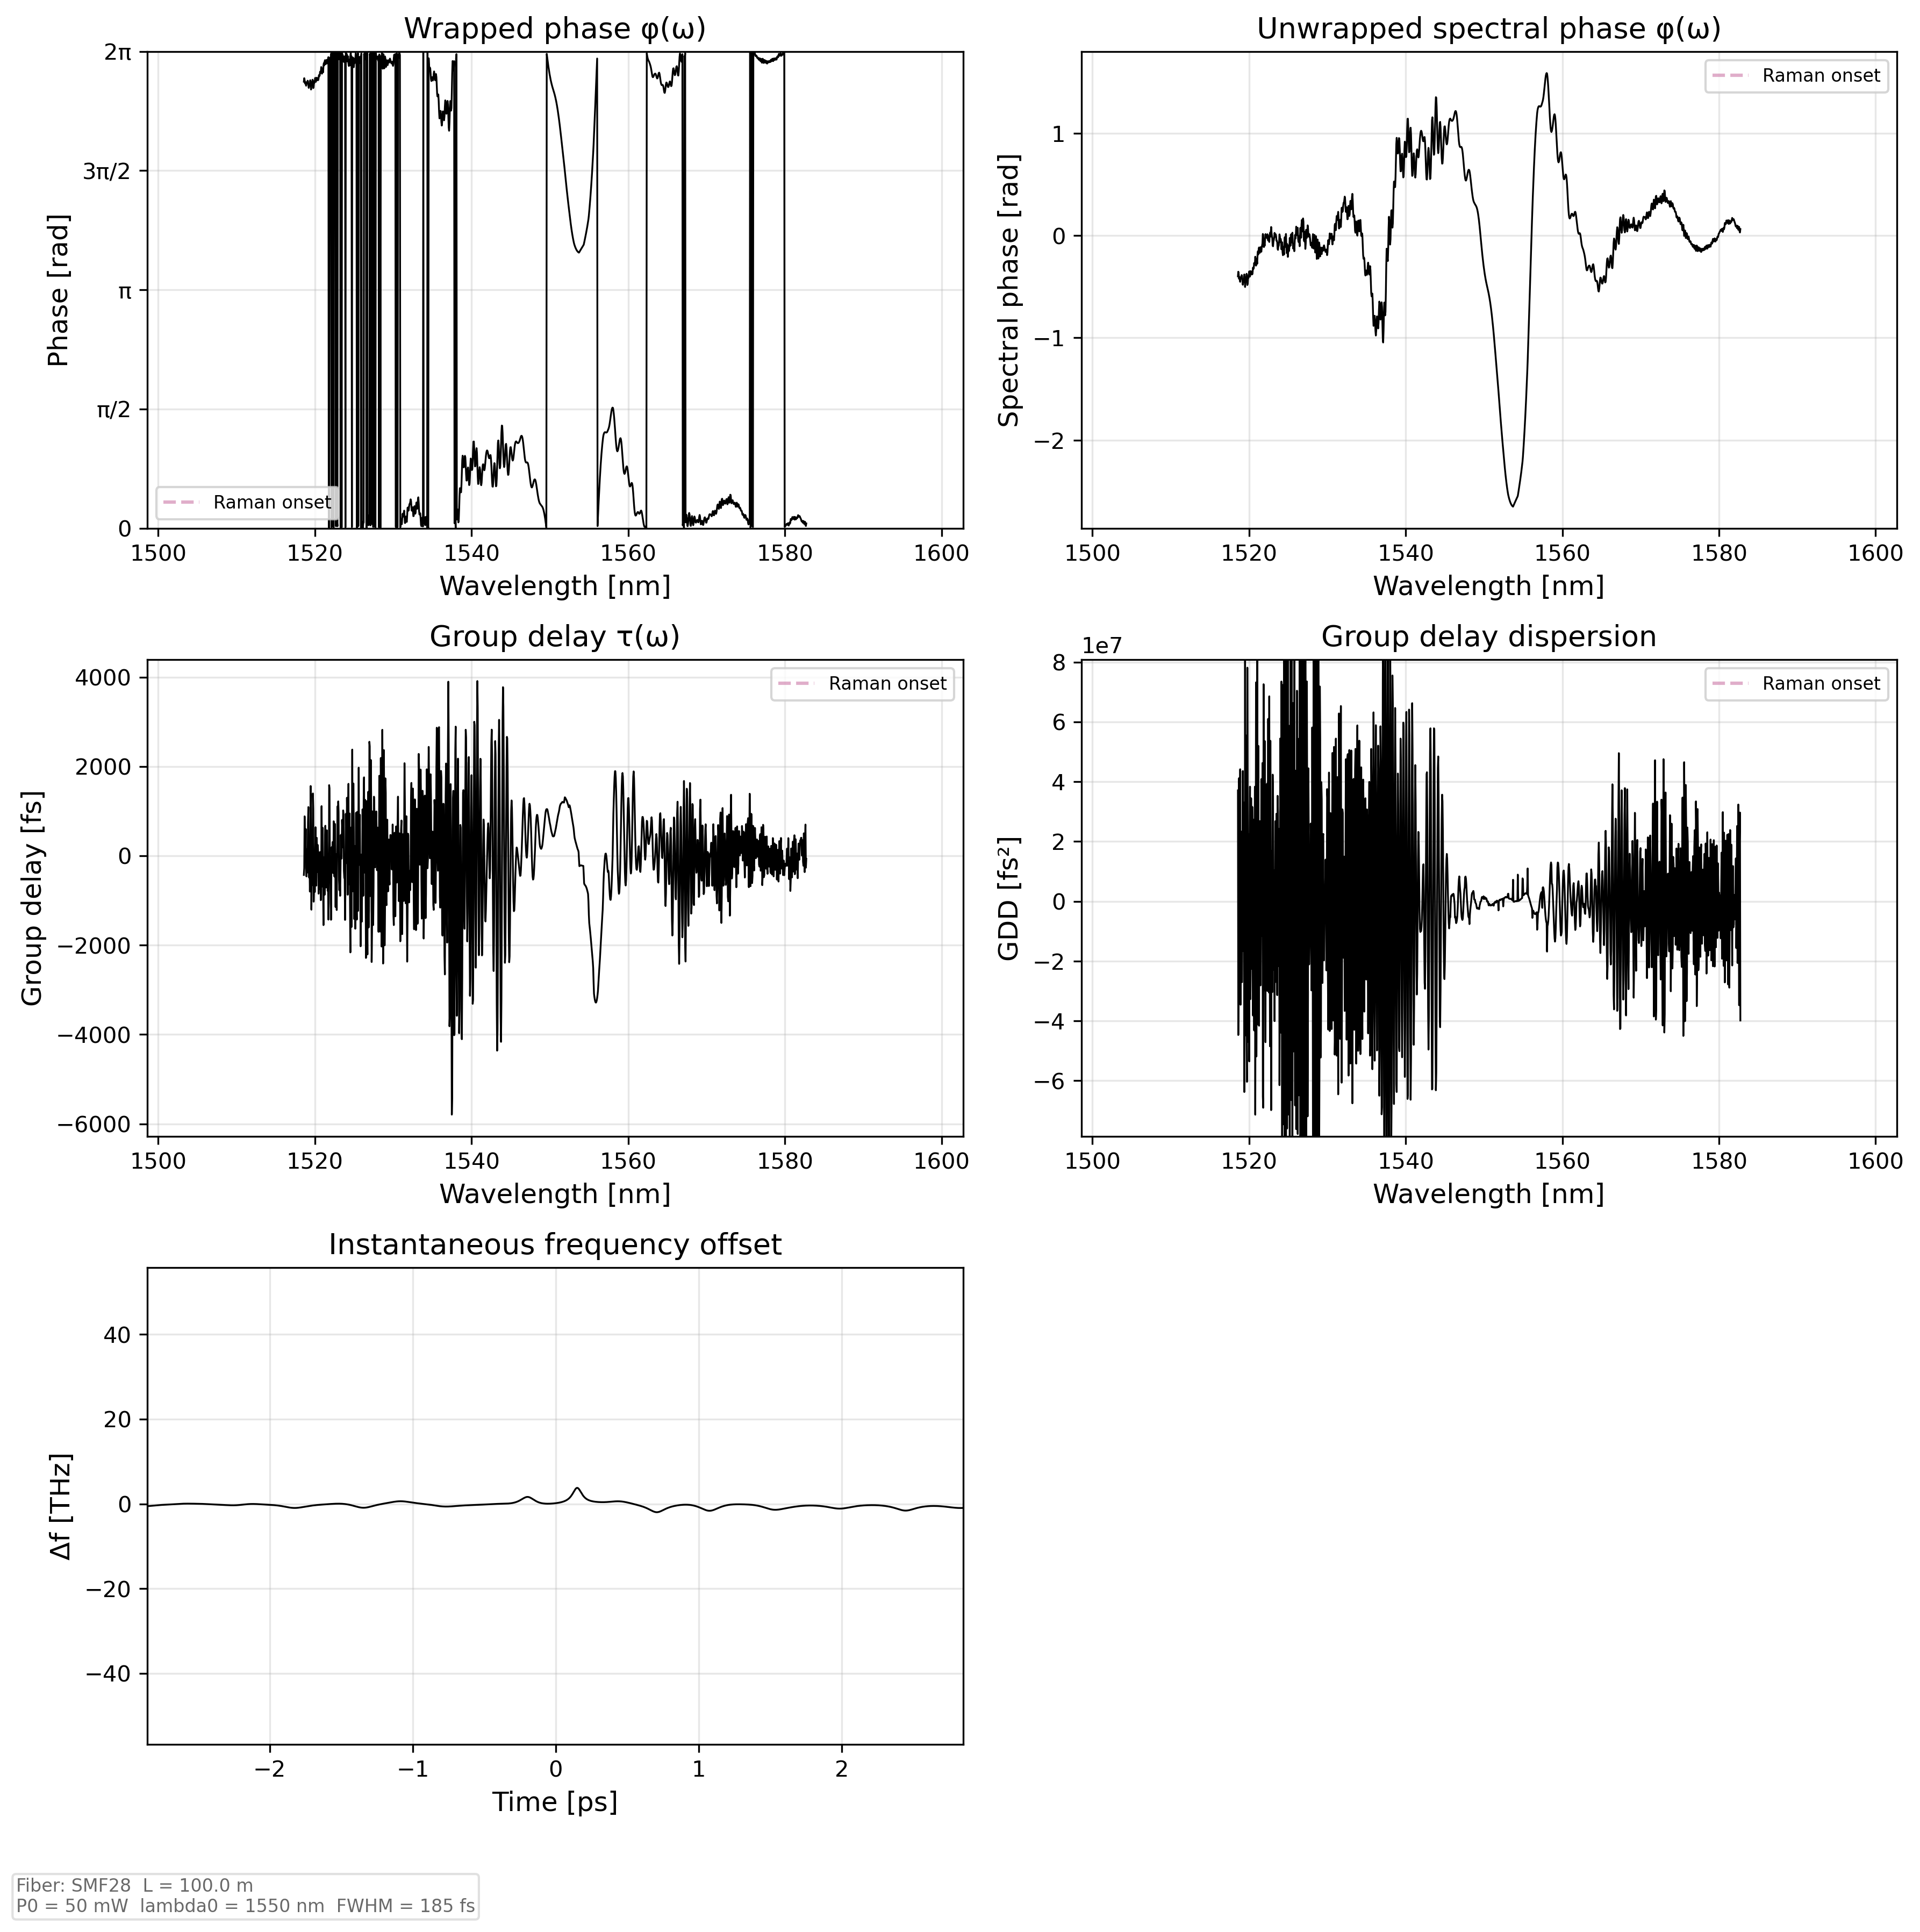
\includegraphics[height=0.47\textheight]{figures/longfiber_100m_phase_diagnostic.png}
\vspace{0.5em}

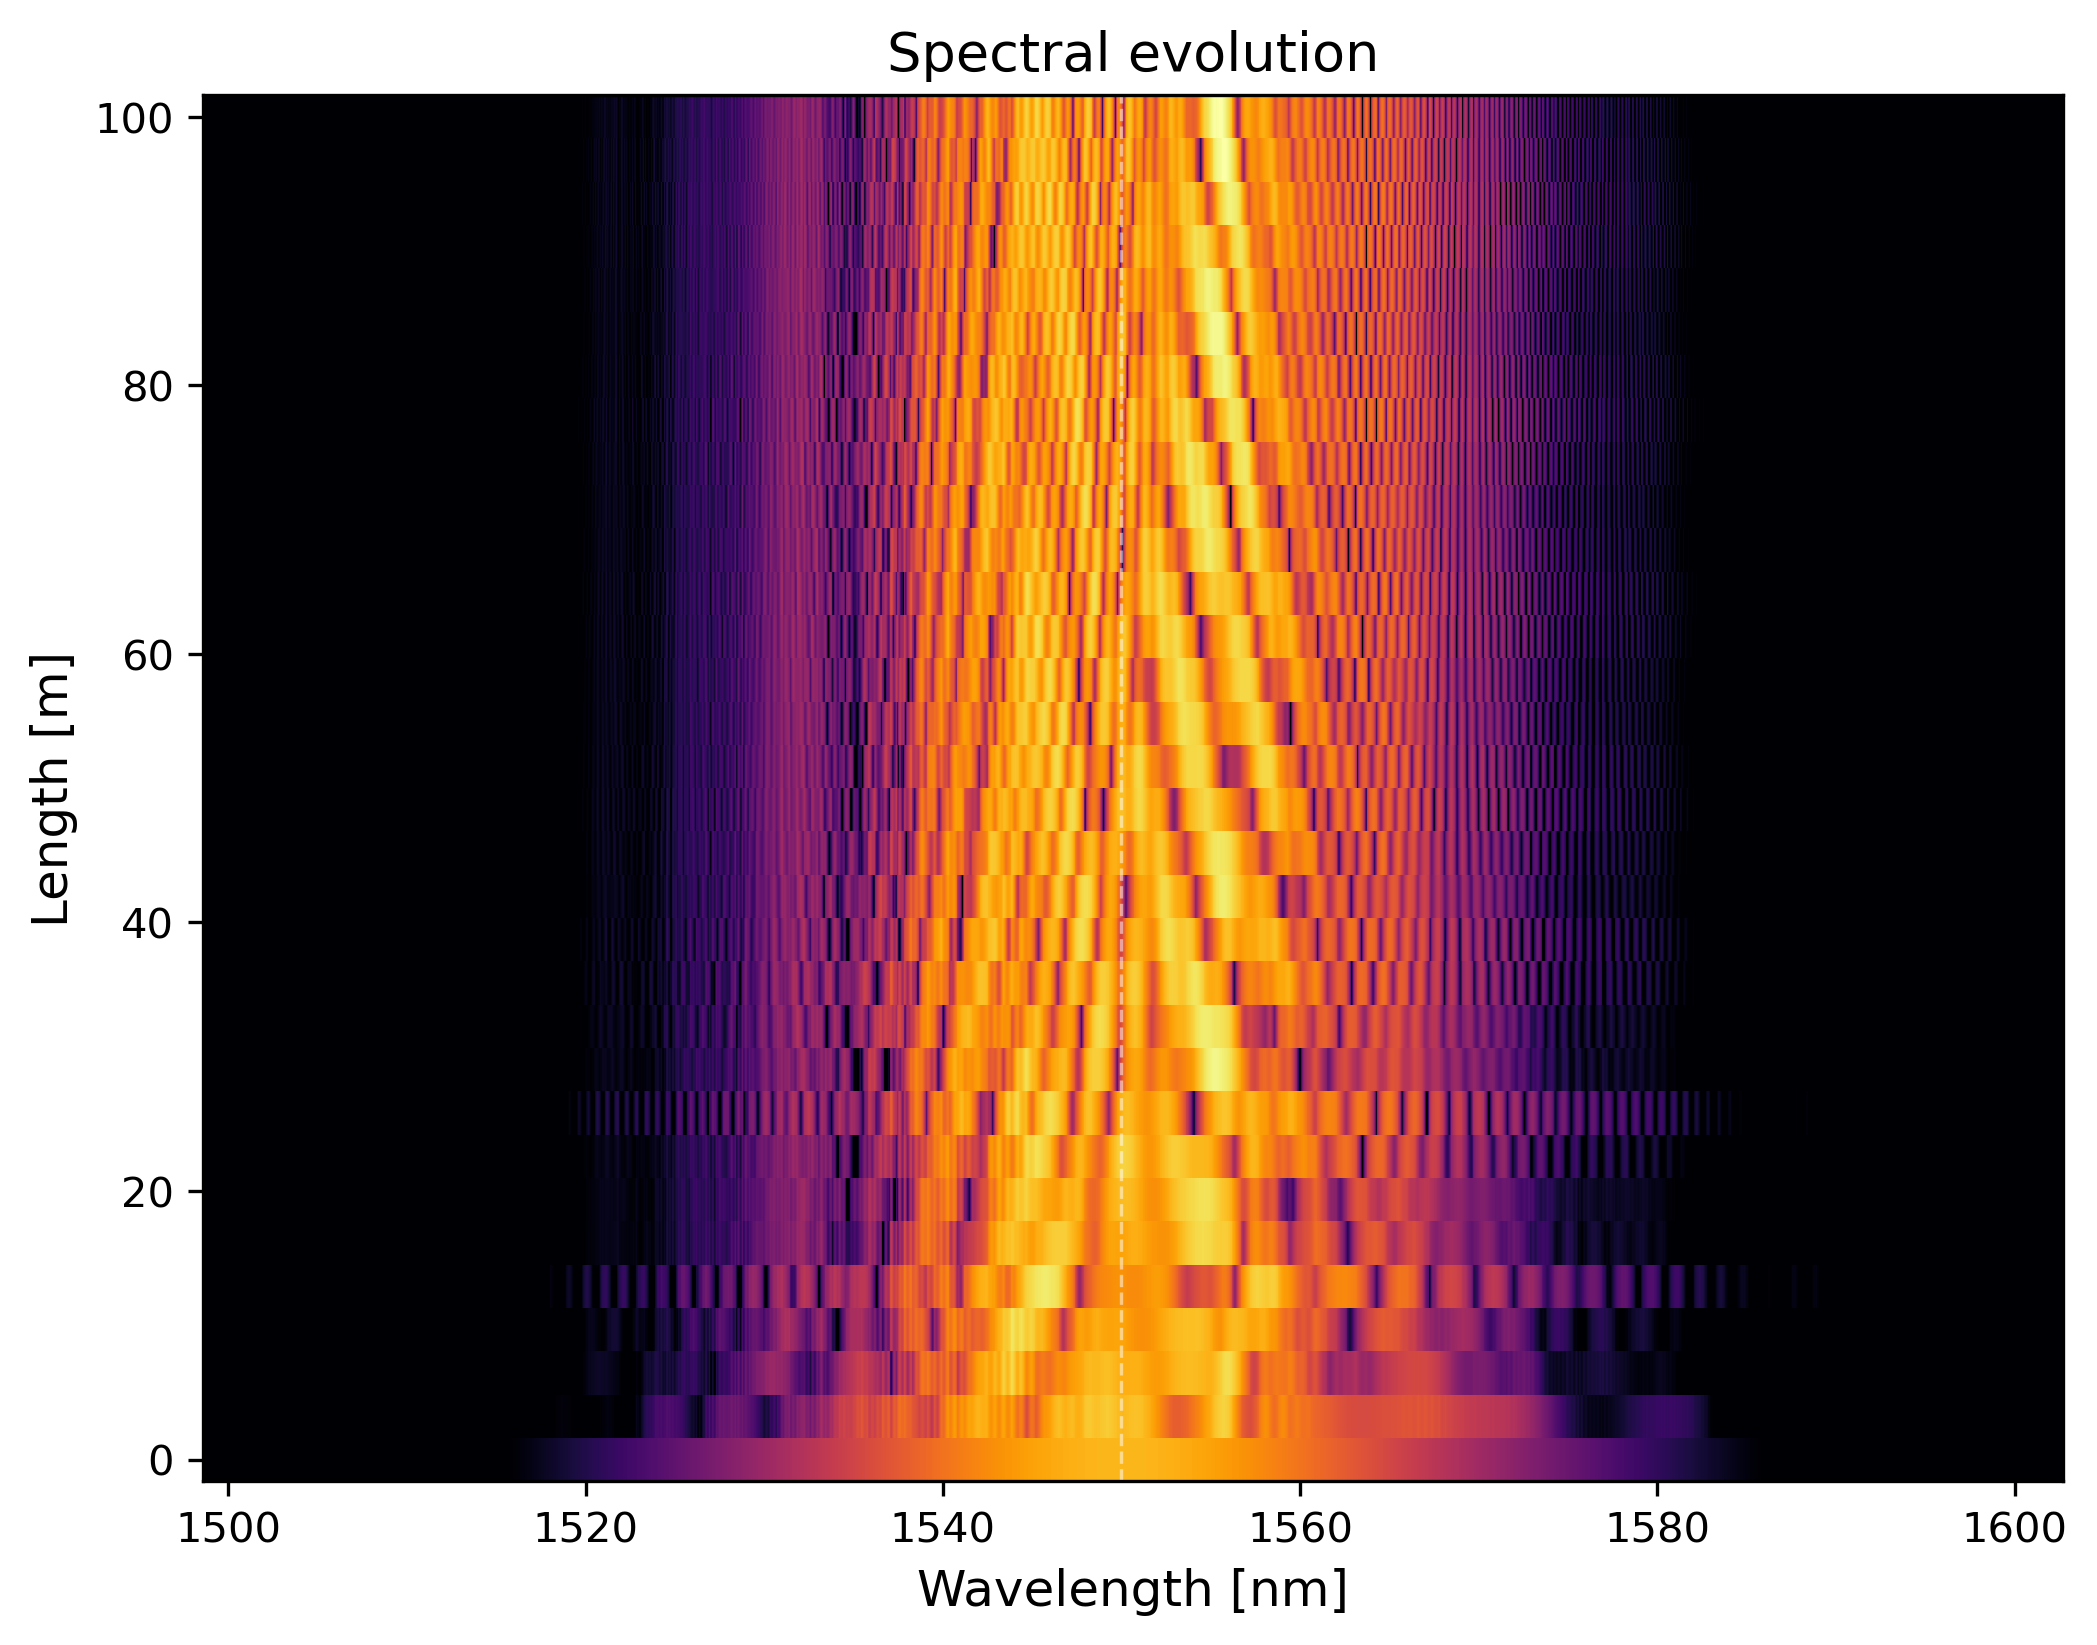
\includegraphics[height=0.31\textheight]{figures/longfiber_100m_evolution.png}
\caption{Paired 100 m optimized diagnostic and heat map. The phase is effective
but not simple; the diagnostic and group-delay curves should be read as a
research result, not as a ready-to-load lab prescription. The matching heat map
shows the propagation response produced by that same mask.}
\end{figure}

\section{200 m Result}

\begin{table}[H]
\centering
\small
\begin{tabular}{@{}lr@{}}
\toprule
\textbf{Quantity} & \textbf{Accepted 200 m resumed result} \\
\midrule
Fiber length & \(200.0\,\mathrm{m}\) \\
Power & \(0.05\,\mathrm{W}\) \\
Grid & \(N_t=65536\), \(320\,\mathrm{ps}\) \\
Final Raman-band fraction & \(-55.1648\,\mathrm{dB}\) \\
Converged flag & false \\
Residual gradient & \(0.5649\) \\
Standard image set & complete and visually inspected \\
\bottomrule
\end{tabular}
\caption{The 200 m result is a completed milestone, not a converged optimum.}
\end{table}

\begin{figure}[H]
\centering
\begin{minipage}{0.48\linewidth}
\centering
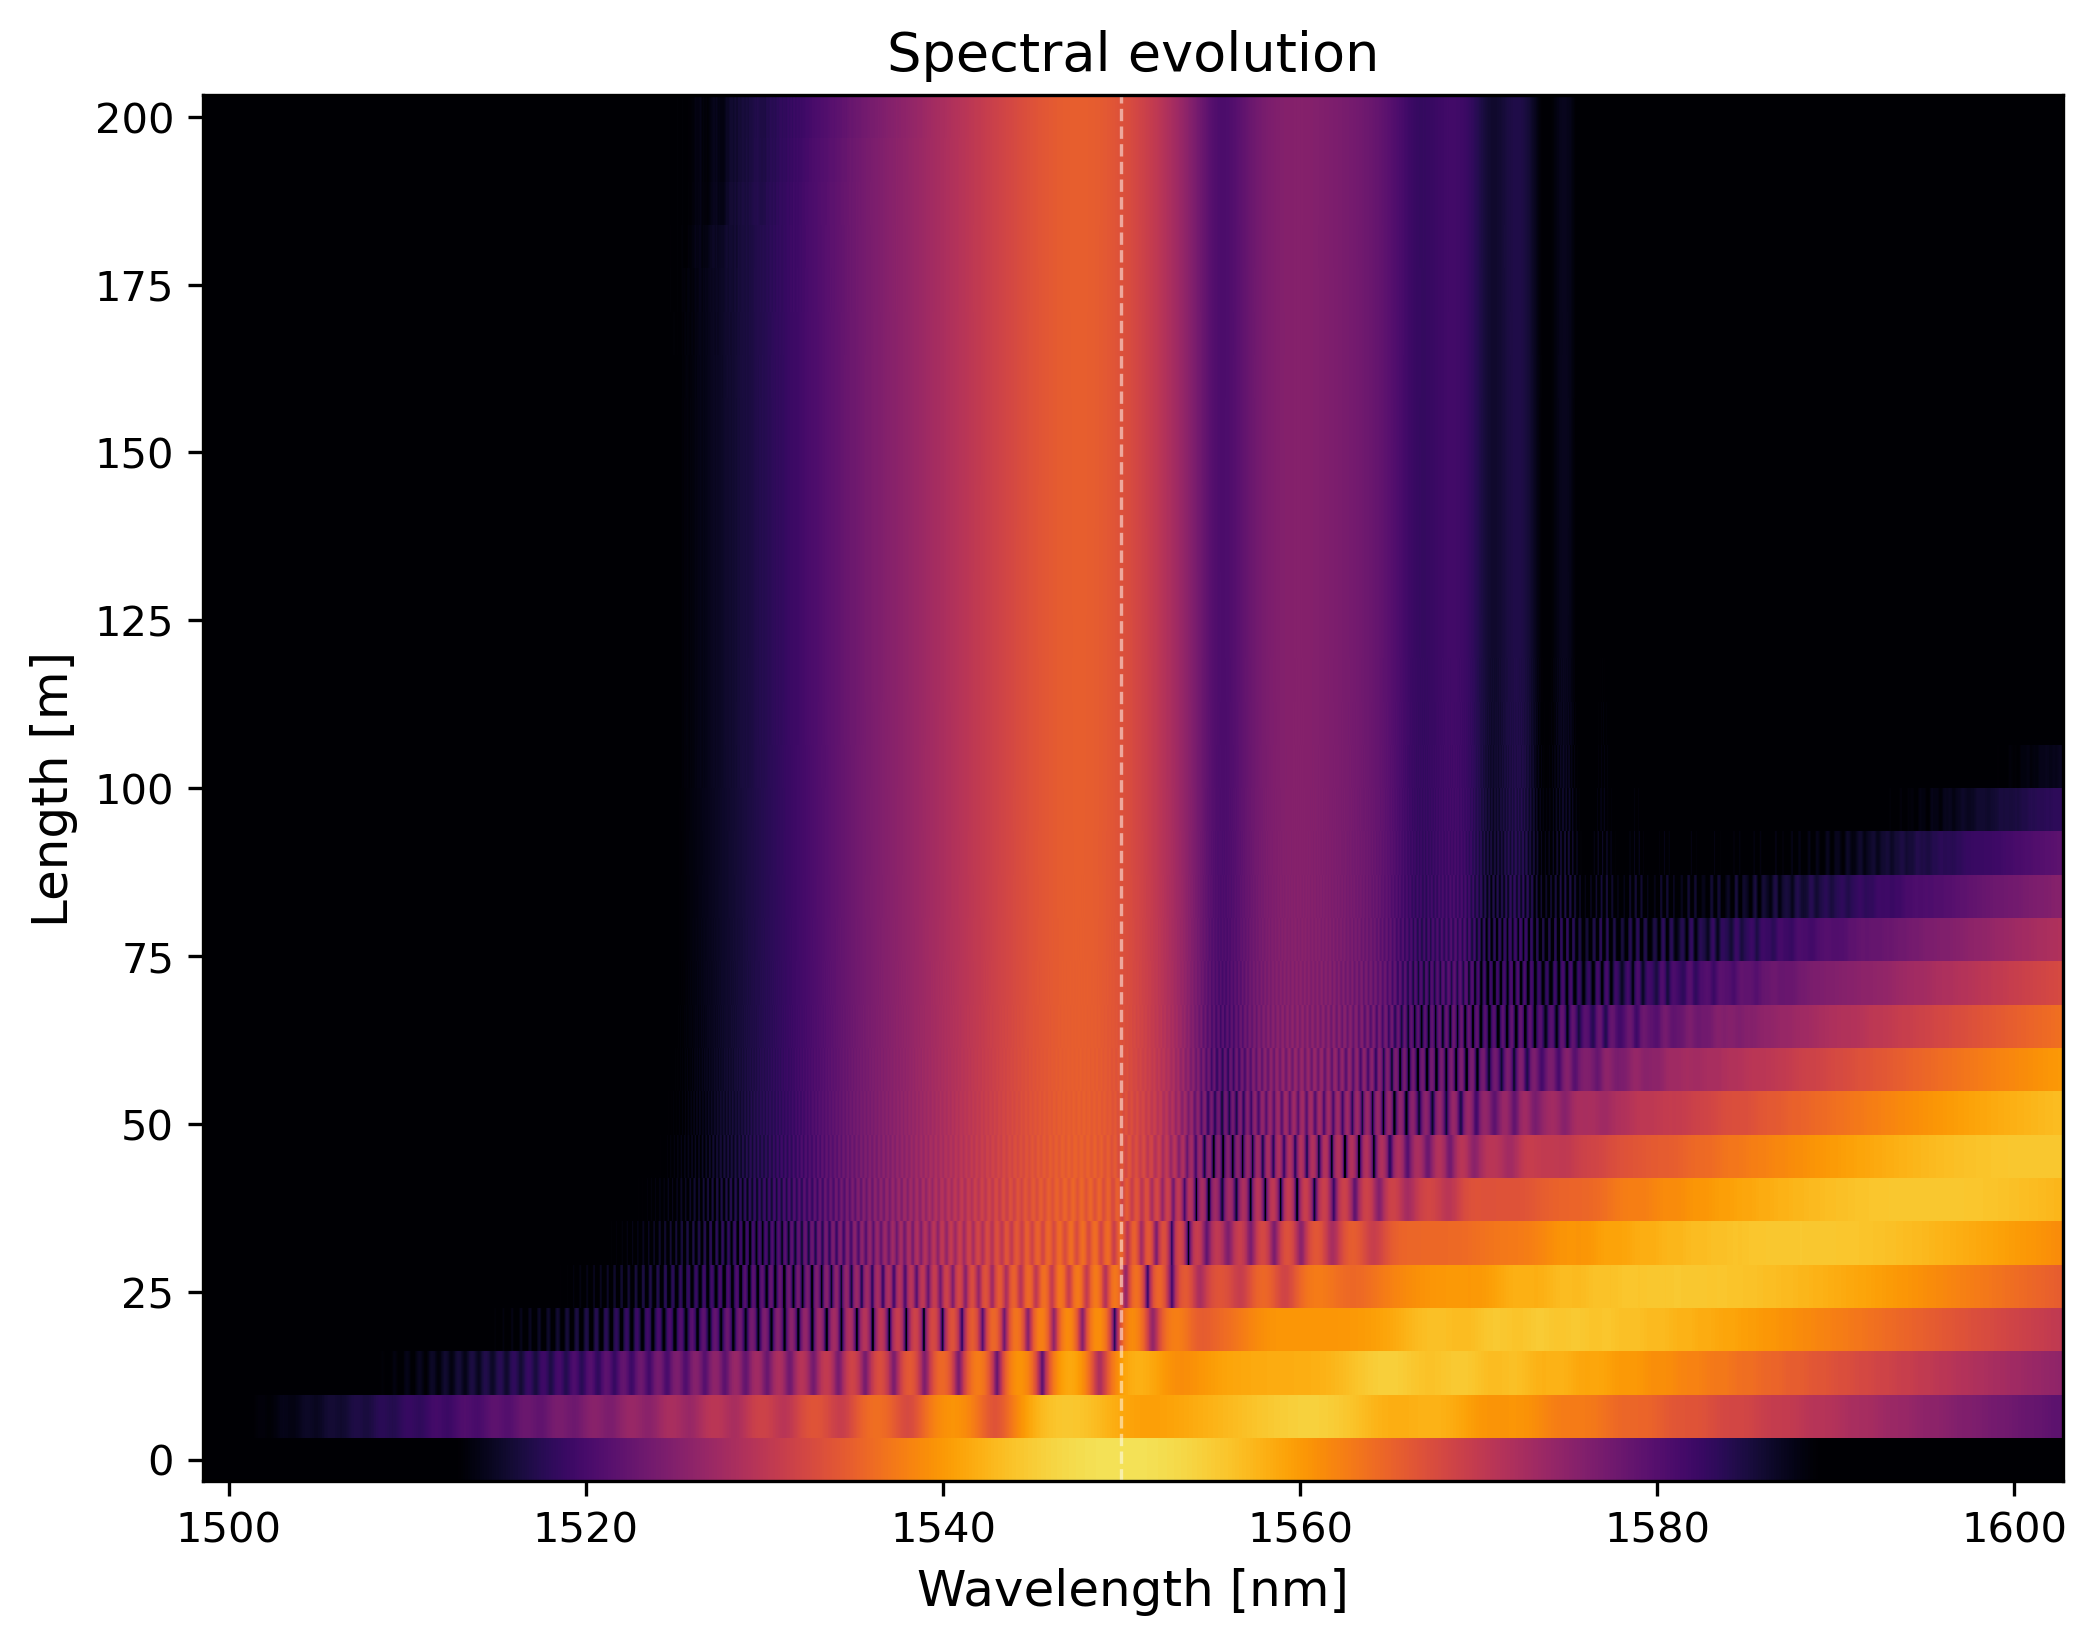
\includegraphics[width=\linewidth]{figures/longfiber_200m_evolution_unshaped.png}
\caption*{200 m no-shaping control.}
\end{minipage}
\hfill
\begin{minipage}{0.48\linewidth}
\centering
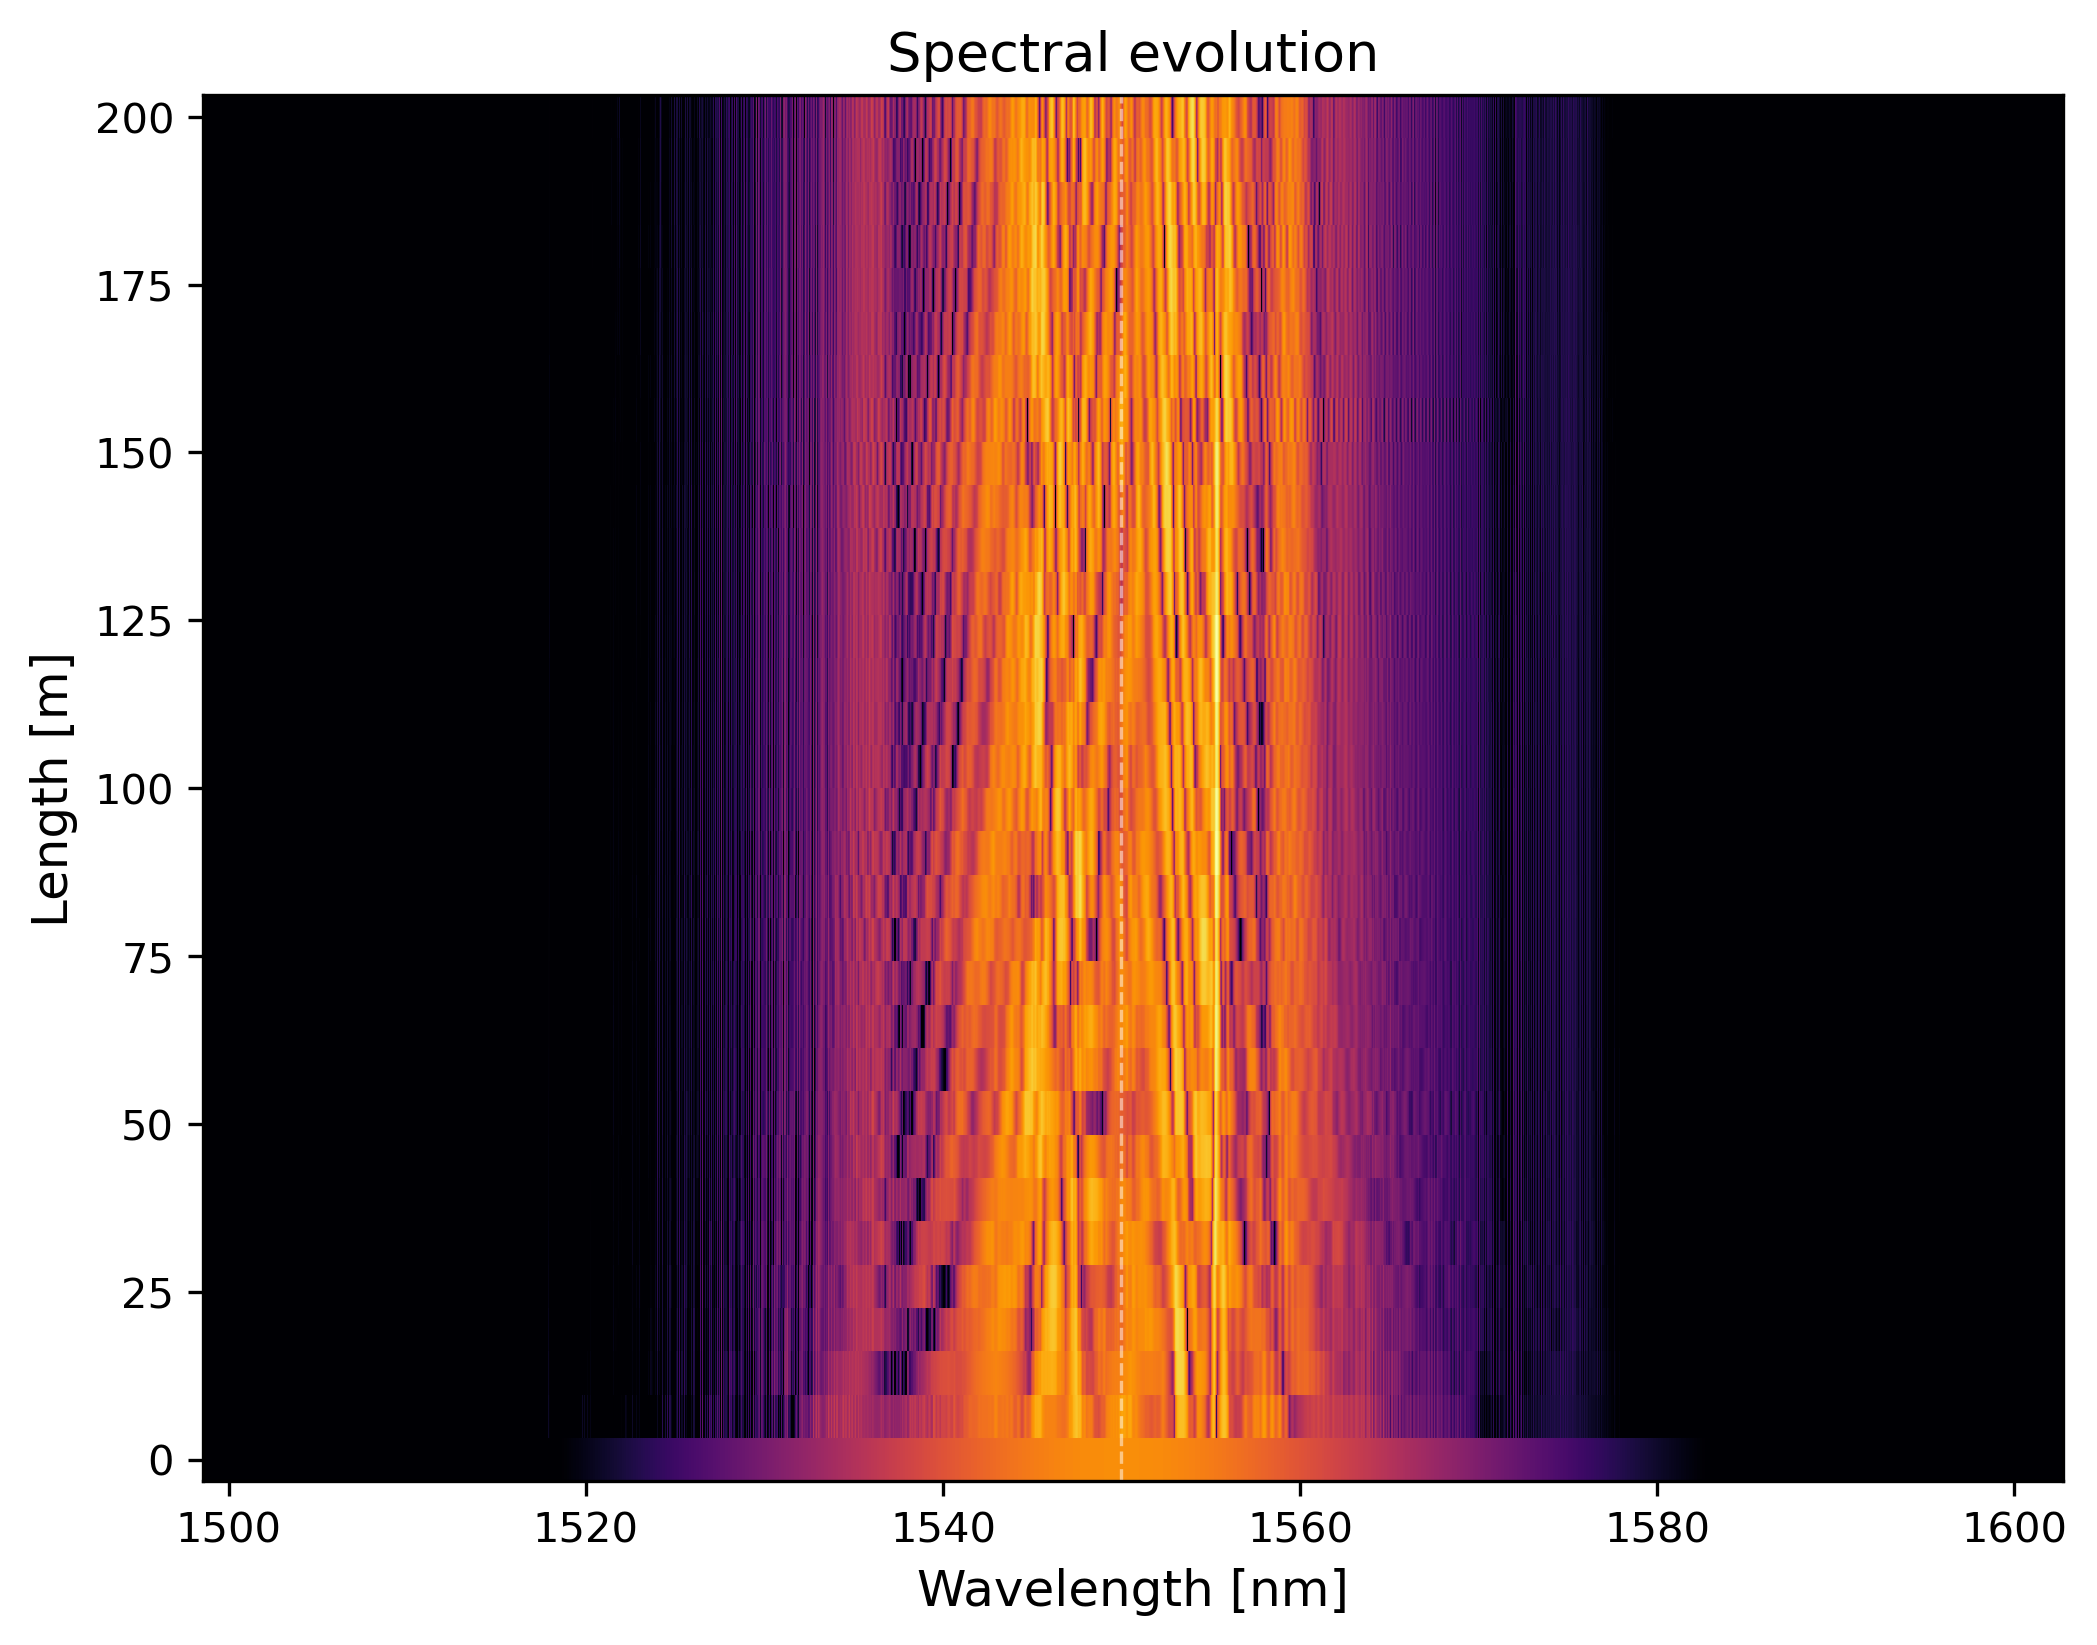
\includegraphics[width=\linewidth]{figures/longfiber_200m_evolution.png}
\caption*{200 m optimized heat map.}
\end{minipage}
\caption{The 200 m standard images show strong suppression of the Raman-side
feature relative to the no-shaping control.}
\end{figure}

\begin{figure}[H]
\centering
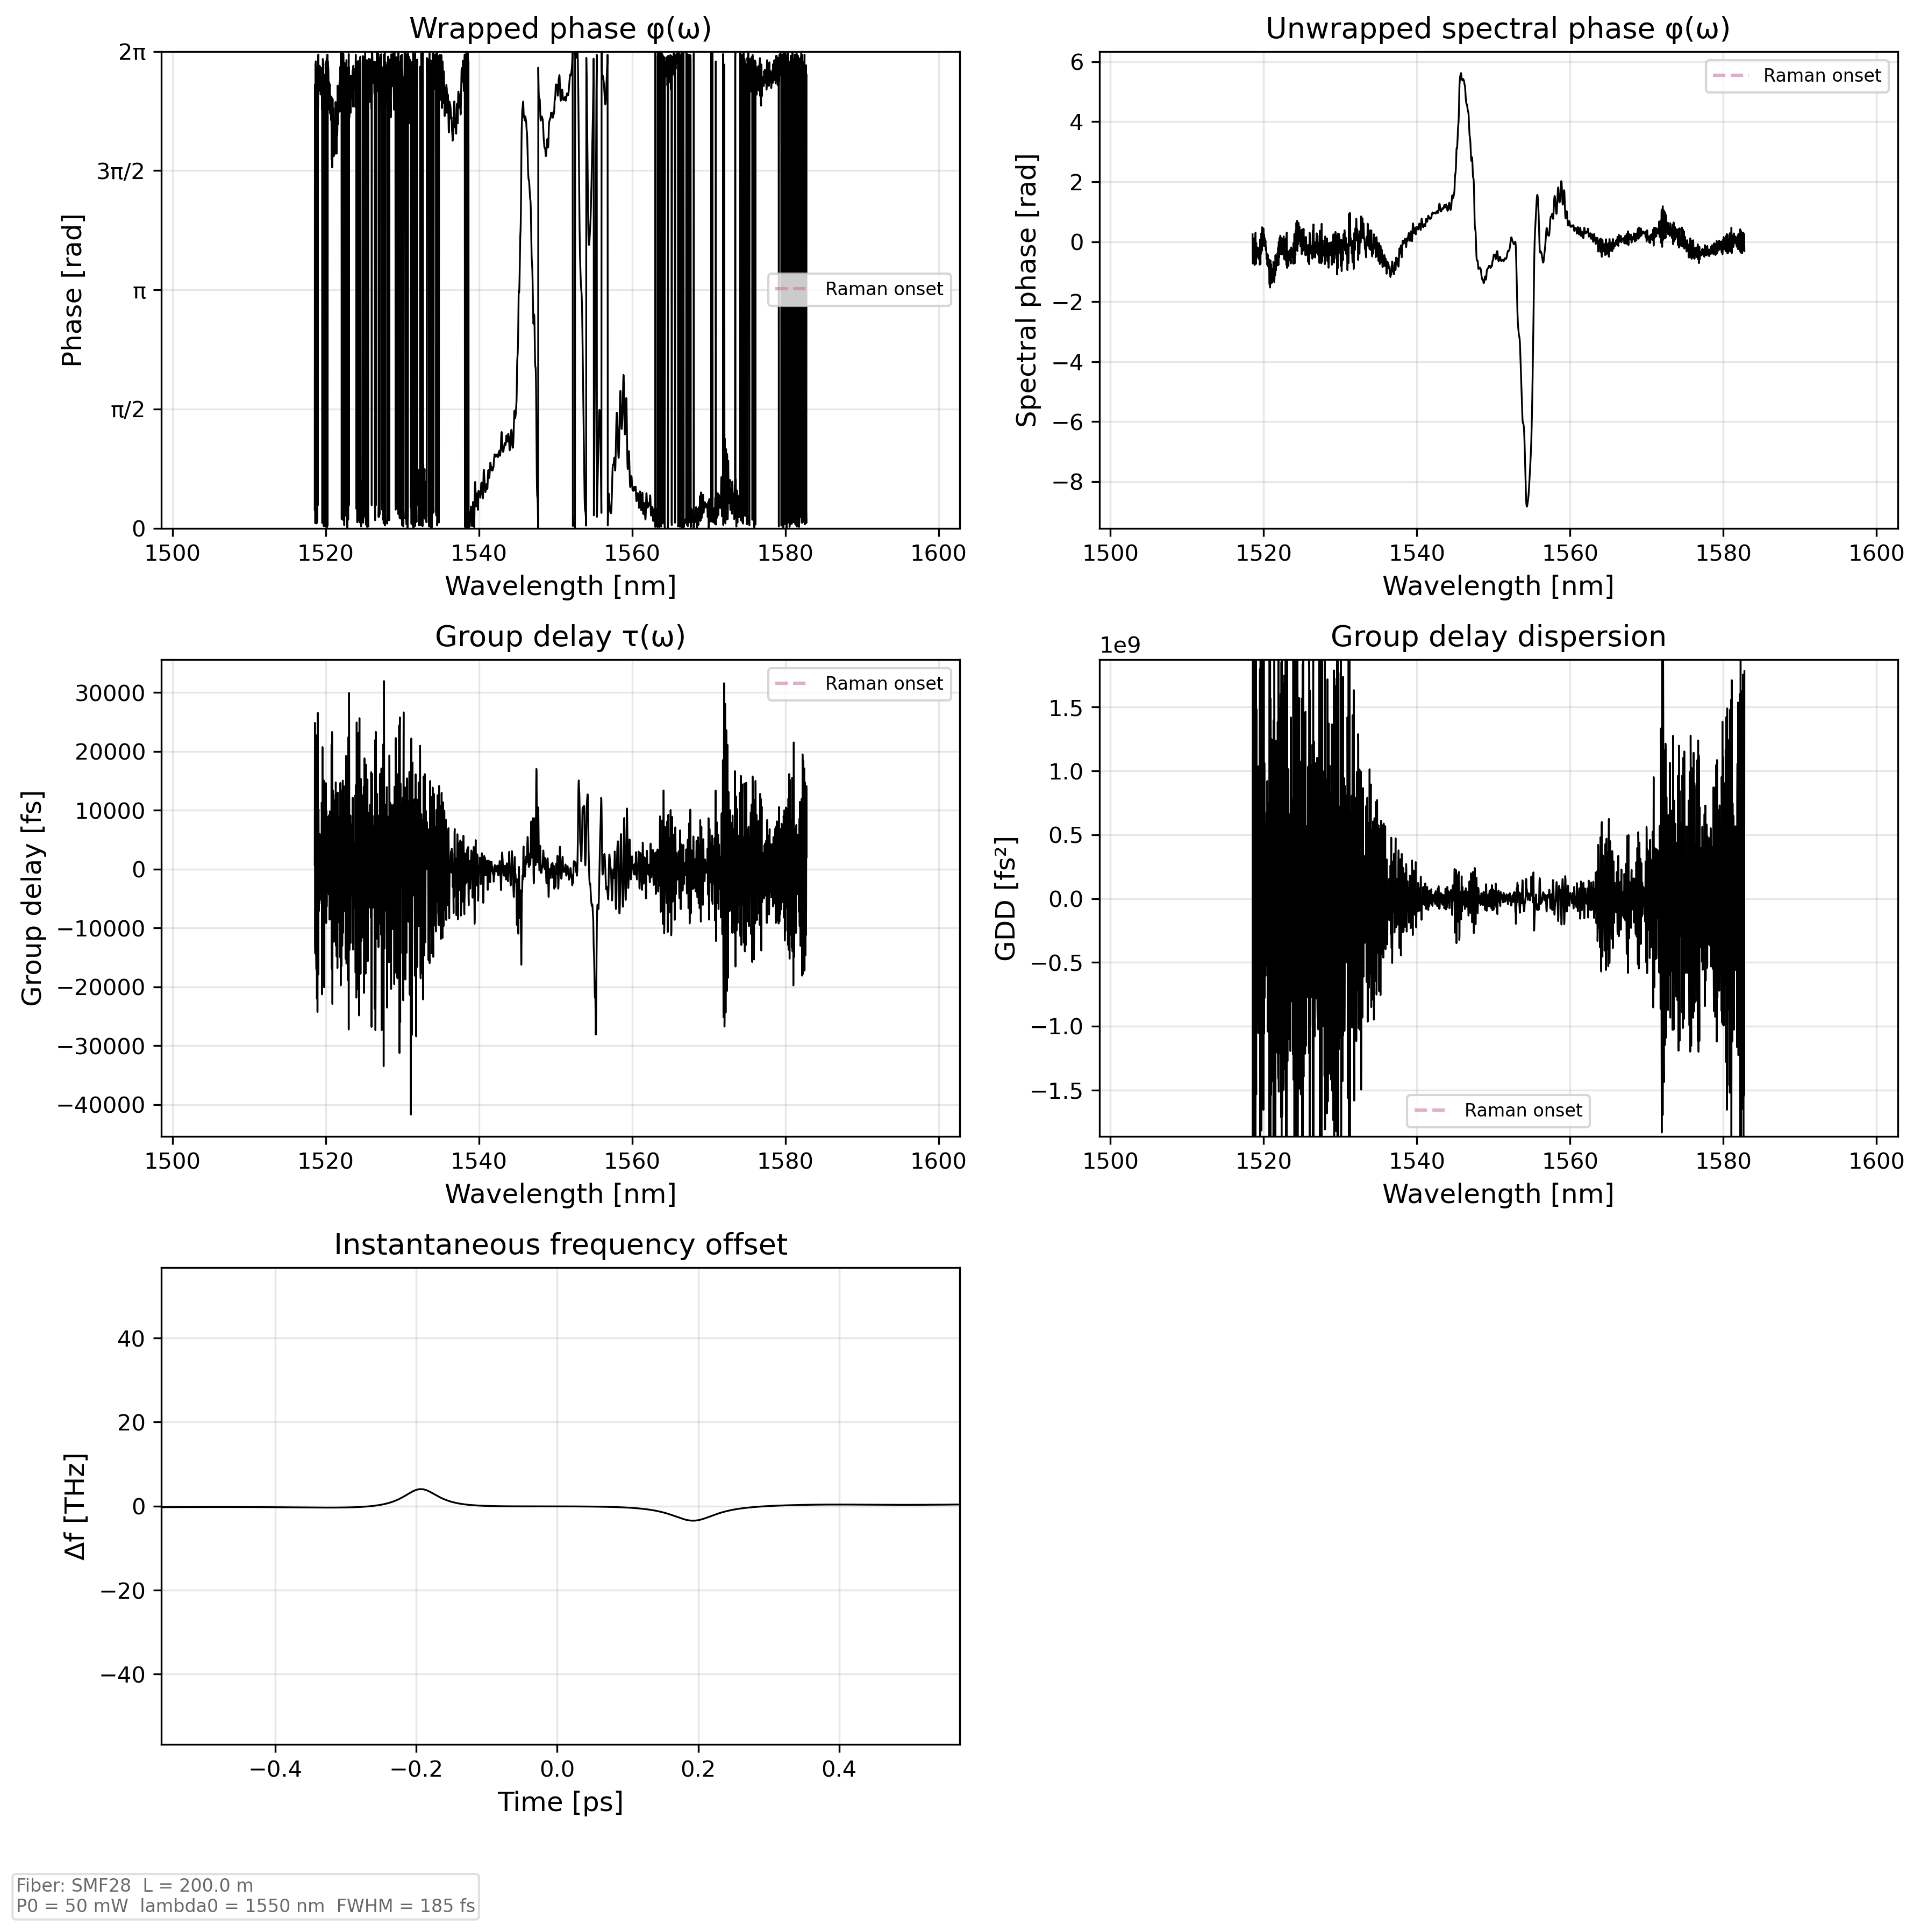
\includegraphics[height=0.47\textheight]{figures/longfiber_200m_phase_diagnostic.png}
\vspace{0.5em}

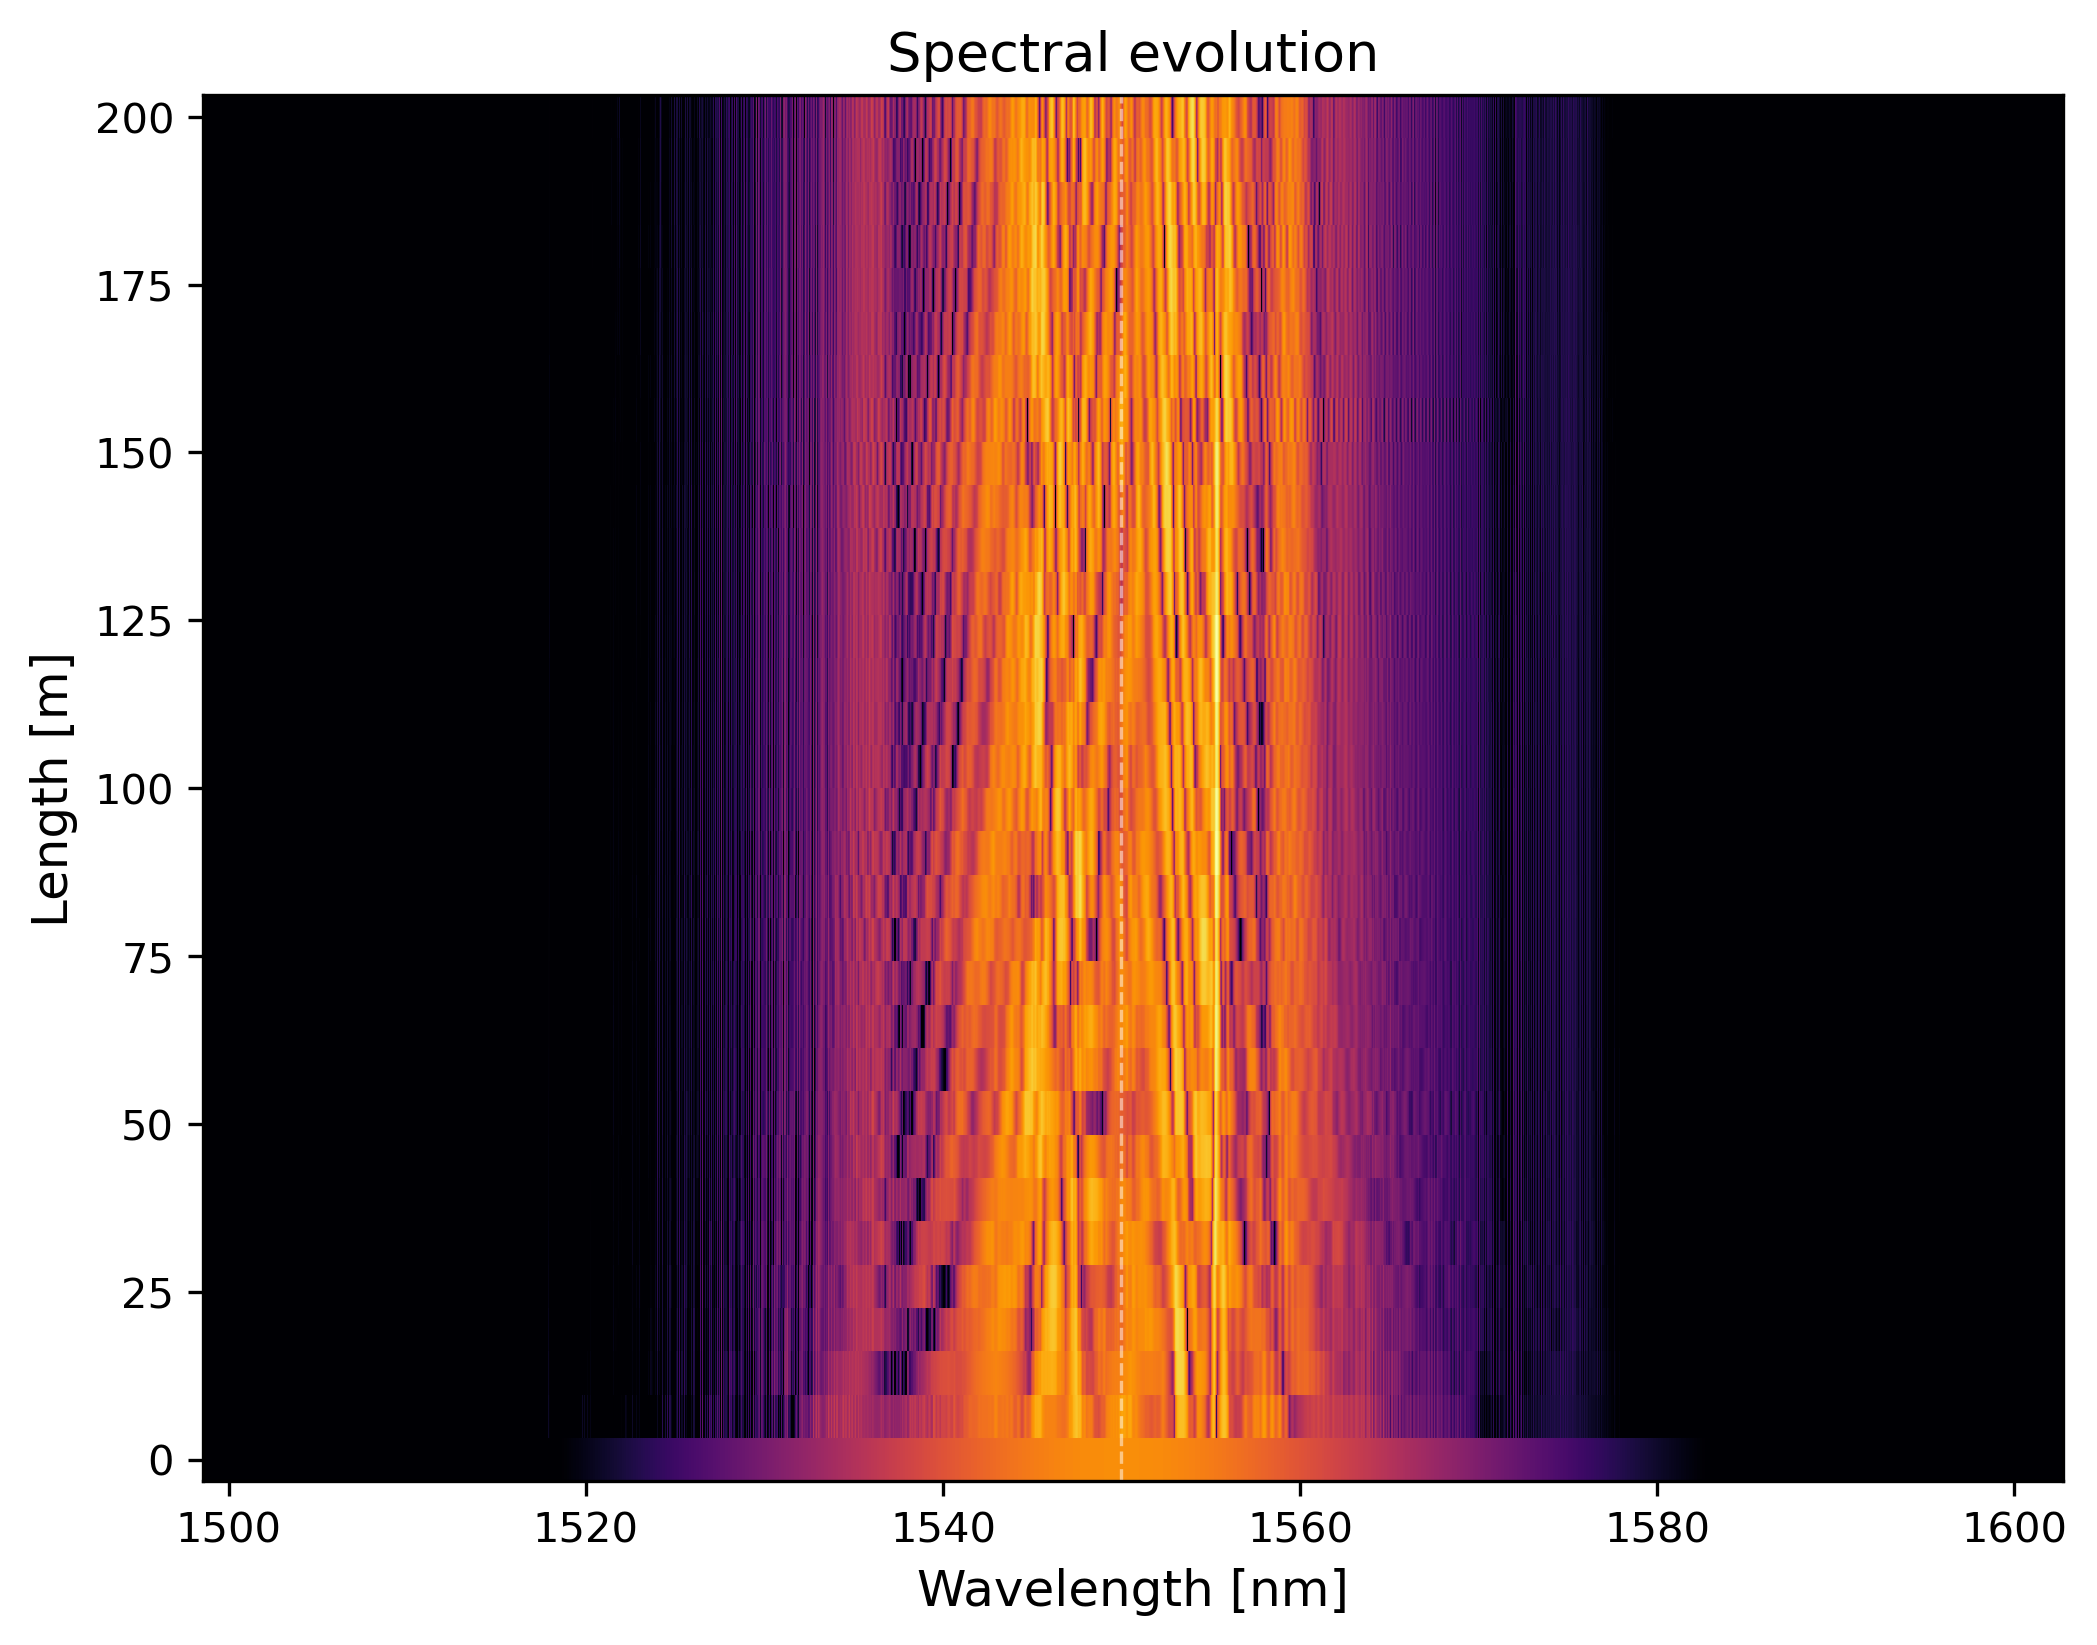
\includegraphics[height=0.31\textheight]{figures/longfiber_200m_evolution.png}
\caption{Paired 200 m optimized diagnostic and heat map. The phase is
high-structure and not actuator-ready. The main claim is that the long-fiber
optimization path reached a deep, visually coherent simulation result.}
\end{figure}

\FloatBarrier

\section{Interpretation}

The long-fiber story has three parts. First, phase shaping can still strongly
alter Raman transfer far beyond the 2 m baseline. Second, the warm-start seed
contains useful structure: before long-fiber reoptimization, it already lands
near the deep-suppression regime. Third, the long-fiber optimized phases are
not simple quadratic pre-chirps. The saved quadratic-fit checks found poor
weighted polynomial fit quality, which means the useful structure is not just
``multiply the dispersion length by a constant.''

\subsection*{TL;DR}

The long-fiber lane is a proof of reach and workflow: the project can carry
phase-only Raman suppression into 100--200 m simulations. It is not yet a proof
that the final saved phase is the simplest, most robust, or globally optimal
long-fiber waveform.

\section{Presentation Capsule}

If this note becomes a presentation block, the clean message is:
\begin{itemize}
    \item The long-fiber result is a scale-up of the same Raman-band objective,
    not a different cost function.
    \item The 100 m and 200 m heat maps are strong before/after visuals because
    the no-shaping controls show obvious Raman growth.
    \item The compute story matters: explicit grids, warm starts, checkpoints,
    and standard images are what made the result usable.
    \item Always include the caveat: these are deep achieved values with
    non-converged optimizer flags, not final global optima.
\end{itemize}

\section{Limitations}

\begin{itemize}
    \item \textbf{Not converged optima.} The accepted 100 m and 200 m results
    have false convergence flags and nontrivial residual gradients.
    \item \textbf{Single-mode only.} This note does not validate multimode
    long-fiber optimization.
    \item \textbf{High-structure phases.} The optimized phases are not simple
    lab-ready actuator prescriptions.
    \item \textbf{Workflow maturity.} The path is usable for research, but not
    yet a turnkey group-facing long-fiber platform.
    \item \textbf{Grid dependence.} Long-fiber claims must name \(N_t\), time
    window, length, power, and validation images.
\end{itemize}

\section{Reproduction Capsule}

Substantial long-fiber runs belong on the heavy compute machine with Julia
threading enabled. The 200 m-style command pattern is:
\begin{verbatim}
LF100_MODE=fresh \
LF100_L=200 \
LF100_NT=65536 \
LF100_TIME_WIN=320 \
LF100_RUN_LABEL=longfiber_200m \
LF100_MAX_ITER=15 \
julia -t auto --project=. scripts/research/longfiber/longfiber_optimize_100m.jl
\end{verbatim}

The expected durable outputs are:
\begin{itemize}
    \item checkpoint directory under the long-fiber results tree;
    \item final result payload;
    \item phase profile image;
    \item phase diagnostic image;
    \item optimized spectral-evolution heat map;
    \item unshaped-control spectral-evolution heat map.
\end{itemize}

Before presenting a new long-fiber result, visually inspect the standard image
set and record the final dB value, convergence flag, residual gradient, grid,
time window, edge fraction, and energy drift.

\section{Sources}

\begin{thebibliography}{9}

\bibitem{agrawal2019}
G. P. Agrawal.
\textit{Nonlinear Fiber Optics}, 6th ed.
Academic Press, 2019.
\url{https://www.sciencedirect.com/book/9780128170427/nonlinear-fiber-optics}

\bibitem{dudley2006}
J. M. Dudley, G. Genty, and S. Coen.
``Supercontinuum generation in photonic crystal fiber.''
\textit{Reviews of Modern Physics}, 78, 1135--1184, 2006.
\url{https://doi.org/10.1103/RevModPhys.78.1135}

\bibitem{hult2007}
J. Hult.
``A Fourth-Order Runge--Kutta in the Interaction Picture Method for
Simulating Supercontinuum Generation in Optical Fibers.''
\textit{Journal of Lightwave Technology}, 25(12), 3770--3775, 2007.
\url{https://doi.org/10.1109/JLT.2007.909373}

\end{thebibliography}

\end{document}
